% ML-driven PVT-variation-aware leakage estimation, PTM 22 nm HP -- IEEE conference format, final version.
% Numbers come only from the saved result files (see docs/REPORT_NOTES.md); every table and number carries a "% src:" comment.
\documentclass[conference]{IEEEtran}
\IEEEoverridecommandlockouts
\usepackage{graphicx}
\usepackage{booktabs}
\usepackage{amsmath,amssymb}
\usepackage{siunitx}
\usepackage{cite}
\usepackage{url}
\usepackage{tikz}
\usetikzlibrary{arrows.meta,positioning,calc,fit,backgrounds}
\sisetup{exponent-product=\times}
\usepackage[hidelinks]{hyperref}   % last

% shrink a table only if it is wider than the column
\newsavebox{\tabbox}
\newcommand{\fitcol}[1]{\sbox{\tabbox}{#1}\ifdim\wd\tabbox>\columnwidth\resizebox{\columnwidth}{!}{\usebox{\tabbox}}\else\usebox{\tabbox}\fi}

% Author layout: 2 x 2 blocks of equal width; \linebreakand starts a new row of author blocks
\newlength{\authorcolwidth}\setlength{\authorcolwidth}{0.36\textwidth}
\makeatletter
\newcommand{\linebreakand}{\end{@IEEEauthorhalign}\hfill\mbox{}\par\mbox{}\hfill\begin{@IEEEauthorhalign}}
\makeatother

% Switches for optional material (true = include)
\newif\ifexpFirstModels \expFirstModelstrue   % first model set, benchmark, components model (Sec. V-C)
\newif\ifexpSymmetry    \expSymmetrytrue      % drain-source symmetry test (Sec. V-F)
\newif\ifexpDist        \expDisttrue          % appendix: current-magnitude distribution
\newif\ifexpFamilies    \expFamiliestrue      % appendix: per-family gate accuracy (comparison only)

\begin{document}
\title{Hierarchical ML-Based Leakage Estimation Under PVT Variation in 22\,nm CMOS}
\author{%
\IEEEauthorblockN{\makebox[\authorcolwidth]{Mididoddi Sai Poojith}}
\IEEEauthorblockA{Roll no.\ 2025122010\\ mididoddi.poojith@research.iiit.ac.in}
\and
\IEEEauthorblockN{\makebox[\authorcolwidth]{Devang Bordoloi}}
\IEEEauthorblockA{Roll no.\ 2025122003\\ devang.bordoloi@research.iiit.ac.in}
\linebreakand
\IEEEauthorblockN{\makebox[\authorcolwidth]{Vajrapu Venkata Sai Aneesh}}
\IEEEauthorblockA{Roll no.\ 2025122002\\ aneesh.vajrapu@research.iiit.ac.in}
\and
\IEEEauthorblockN{\makebox[\authorcolwidth]{Apanna Nihaal}}
\IEEEauthorblockA{Roll no.\ 2025122007\\ nihaal.appana@research.iiit.ac.in}
\linebreakand
\IEEEauthorblockA{\textbf{Team Dvd Angels}\\ International Institute of Information Technology Hyderabad, India}}
\maketitle

\begin{abstract}
We estimate the leakage current of CMOS logic gates and of a 3-bit carry-lookahead adder (CLA) under process, voltage and temperature (PVT) variation with machine-learning models instead of SPICE, for the PTM 22\,nm high-performance technology at a nominal supply of 1\,V.
Four transistor-level models (NMOS and PMOS, ON and OFF) predict the four terminal currents of a single transistor from 10,000 SPICE samples per case; each is chosen from four model types (Gaussian process, hybrid analytical\,+\,MLP, residual MLP, physics-informed network) on a validation set of an 80:10:10 split.
Using only these models and the recorded SPICE node voltages, the gate leakage is assembled with Kirchhoff's current law on the supply node.
Over 3,600 gate simulations (five gates, 18 input cases, 200 corners) the mean accuracy is 98.87\,\% (median 99.18\,\%); the plain sum of the 33 gate leakages predicts the adder leakage over 12,800 simulations (64 vectors, 200 corners) with a mean accuracy of 99.00\,\% (median 99.17\,\%).
The 99\,\% target is therefore met for the circuit but not for the gates, and the circuit result benefits from a cancellation: summing isolated gate leakages alone caps the adder accuracy at 99.16\,\% even with perfect gate models.
The remaining gate error is concentrated in OFF transistors operated with the full supply across them, a corner of the input space that uniform sampling covers with less than 0.5\,\% of the training rows.
We also report the negative results that shaped the method: a silent \texttt{altermod} bug in the data generation, a plain current sum that fails by orders of magnitude, and a drain--source symmetry that the device model does not have.
% src: results/partB/gate_results.csv, results/partC/cla3_results.csv, results/analysis/report_numbers/rail_point_row_counts.csv; docs/REPORT_NOTES.md sections 7, 8, 9.1
\end{abstract}
\begin{IEEEkeywords}
leakage estimation, PVT variation, machine learning, BSIM4, logic gates, carry-lookahead adder
\end{IEEEkeywords}
\section{Introduction}\label{sec:intro}
Leakage current is a large part of the power budget of nanometre CMOS circuits and it varies by orders of magnitude with temperature, supply voltage and process parameters such as threshold voltage and oxide thickness~\cite{roy2003}.
Estimating it over many PVT corners with transistor-level SPICE simulation is accurate but slow, because every circuit, input vector and corner needs its own simulation.
A surrogate that predicts the currents of a single transistor from its bias, geometry, temperature and process parameters can be evaluated in microseconds and reused for every circuit built from the same transistors.

This work builds such a hierarchy for the PTM 22\,nm high-performance (HP) model card~\cite{ptm,ptmweb} (BSIM4~\cite{bsim4}) at a nominal supply of 1\,V: \emph{transistor} $\rightarrow$ \emph{gate} $\rightarrow$ \emph{circuit} (Fig.~\ref{fig:flow}).
Four machine-learning models predict the terminal currents $(i_d,i_g,i_s,i_b)$ of an NMOS or PMOS transistor in its ON and OFF state. Only these four models are then used to predict the leakage of an inverter, NAND2, NOR2, AND2 and OR2 for every input combination at 200 random corners, and the leakage of a 3-bit carry-lookahead adder as the sum of its 33 gate leakages; every prediction is compared with a transistor-level SPICE simulation.
The target is a mean accuracy of up to 99\,\%.

\begin{figure}[t]
\centering
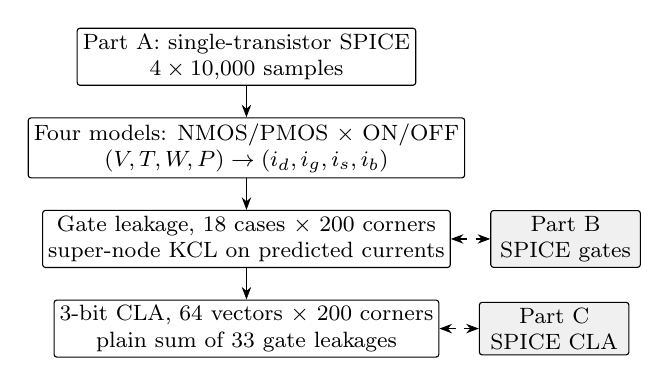
\begin{tikzpicture}[font=\footnotesize,
  box/.style={draw,rounded corners=1pt,align=center,minimum width=4.3cm,inner sep=2pt},
  ref/.style={draw,rounded corners=1pt,align=center,fill=gray!12,minimum width=1.9cm,inner sep=2pt},
  >={Stealth[length=1.6mm]}]
\node[box] (A) {Part A: single-transistor SPICE\\ $4\times 10{,}000$ samples};
\node[box,below=4mm of A] (M) {Four models: NMOS/PMOS $\times$ ON/OFF\\ $(V,T,W,P)\rightarrow(i_d,i_g,i_s,i_b)$};
\node[box,below=4mm of M] (G) {Gate leakage, 18 cases $\times$ 200 corners\\ super-node KCL on predicted currents};
\node[box,below=4mm of G] (C) {3-bit CLA, 64 vectors $\times$ 200 corners\\ plain sum of 33 gate leakages};
\node[ref,right=5mm of G] (GS) {Part B\\ SPICE gates};
\node[ref,right=5mm of C] (CS) {Part C\\ SPICE CLA};
\draw[->] (A)--(M); \draw[->] (M)--(G); \draw[->] (G)--(C);
\draw[<->,dashed] (G)--(GS); \draw[<->,dashed] (C)--(CS);
\end{tikzpicture}
\caption{Transistor $\rightarrow$ gate $\rightarrow$ circuit pipeline. The gray boxes are the SPICE references (evaluation only; never used for training or model selection); dashed arrows are the comparisons.}
\label{fig:flow}
\end{figure}

\textbf{Contributions.}
(i)~A reproducible data-generation flow in which all random draws are made inside ngspice, verified against direct model-card edits (Sec.~\ref{sec:data}).
(ii)~Four transistor models chosen on validation data only from four model types, including a tuning step with a pre-declared selection rule (Sec.~\ref{sec:models}).
(iii)~A Kirchhoff (super-node) construction of the gate leakage from predicted terminal currents, which makes the prediction exact for exact currents, whereas the plain current sum fails (Sec.~\ref{sec:gates}).
(iv)~Gate- and circuit-level accuracy together with a ceiling analysis that separates the error of the models from the error of summing isolated gates (Sec.~\ref{sec:circuit}).
\section{Setup}\label{sec:setup}
Table~\ref{tab:setup} summarises the experimental setup. The test circuit is a 3-bit carry-lookahead adder with six primary inputs (no carry-in, hence 64 input vectors). It is built only from the gates of Part~B: 27 NAND2, 3 inverters, 2 AND2 and 1 OR2, i.e.\ 33 gates and 138 transistors; each XOR is written as four NAND2 and the wide carry terms are split into two-input gates.
% src: partA_transistor/README.md, partB_gates/README.md, partC_cla/README.md, results/partC/cla3_gates.csv, ml/config.py, docs/REPORT_NOTES.md section 1
\begin{table}[t]
\caption{Experimental setup.}
\label{tab:setup}
\centering\footnotesize
\setlength{\tabcolsep}{3pt}
\begin{tabular}{p{2.0cm}p{5.9cm}}
\toprule
Item & Value \\
\midrule
Technology & PTM 22\,nm HP, BSIM4 level 54 (\texttt{22nm\_HP.pm}); $V_{DD}=\SI{1}{\volt}$ nominal, $L=\SI{22}{\nano\meter}$ \\
Sampling & $V_{DD}$ and process parameters (vth0, toxe, ndep, u0, xj) nominal $\pm10\,\%$; $T=-40$--$125\,^\circ$C; $W=1$--$8\,L_{min}$; $V_d,V_s\sim\mathcal U[0,V_{DD}]$ \\
Data & 4 single-transistor datasets $\times$ 10,000 rows (Part~A); 5 gates, 18 input cases $\times$ 200 corners $=$ 3,600 (Part~B); 64 vectors $\times$ 200 corners $=$ 12,800 (Part~C) \\
Simulator & ngspice-44.2 (Windows, \texttt{.op}, one netlist per dataset); \texttt{.options gmin=1e-18 abstol=1e-18 reltol=1e-6 vntol=1e-9}~\cite{ngspice} \\
Models & 4 types (GPR, hybrid, ResNet, PINN); split 80:10:10, split seed 42, model seed 0; SPICE \texttt{rndseed} 12--15 (Part~A), 16 (Parts~B, C) \\
Software & Python 3.12.7, PyTorch 2.14.1~\cite{pytorch}, scikit-learn 1.5.1~\cite{sklearn}, SciPy 1.13.1~\cite{scipy} \\
Hardware & Intel Core i5-12450H (8 cores), 15.7\,GB RAM, NVIDIA RTX 3050 Laptop GPU (4\,GB) \\
Use of data & Part~B and C data are for \emph{evaluation only}: never used for training, tuning or model selection \\
\bottomrule
\end{tabular}
\end{table}
The validation checks of this report were re-run with the ngspice-44 build available under WSL, whose random stream differs from the one of the data build (Sec.~\ref{sec:data:corners}).
% src: validation_checks/corner_build_check.txt, docs/deliverables_check.txt

\section{Data Generation}\label{sec:data}

\subsection{Single-transistor datasets (Part A)}\label{sec:data:gen}
For each case (NMOS ON, NMOS OFF, PMOS ON, PMOS OFF) one ngspice netlist generates 10,000 samples without any external script: a \texttt{.control} loop draws the sample with \texttt{sunif(0)}, applies it with \texttt{alter} (sources, width), \texttt{altermod} (model parameters) and \texttt{option temp}, runs \texttt{.op}, and appends one CSV row with \texttt{echo}. Every terminal has its own voltage source ($V_d,V_g,V_s,V_b$) and the currents are recorded into the terminals. $V_{DD}$ is drawn first because the ranges of $V_d$ and $V_s$ depend on it:
\begin{align}
V_{DD}&\sim\mathcal U[0.9,1.1]\,\text{V},\quad V_d,V_s\sim\mathcal U[0,V_{DD}],\nonumber\\
W&\sim\mathcal U[1,8]\,L_{min},\quad T\sim\mathcal U[-40,125]\,^\circ\text{C},\nonumber\\
p_k&\sim\mathcal U[0.9\,p_k^{nom},\,1.1\,p_k^{nom}],
\end{align}
with $p_k\in\{\text{vth0, toxe, ndep, u0, xj}\}$ drawn separately for NMOS and PMOS around the values of the model file. The gate and body voltages are fixed by the case: ON cases $V_g=V_{DD}$ (NMOS) or 0 (PMOS) with $V_b=0$ or $V_{DD}$; OFF cases $V_g=V_b=0$ (NMOS) or $V_g=V_b=V_{DD}$ (PMOS). SPICE seeds are \texttt{rndseed} 13, 12, 14, 15 for NMOS ON, NMOS OFF, PMOS ON, PMOS OFF.
All sampled values lie inside the bounds above ($V_{DD}$ \SIrange{0.900}{1.100}{\volt}, $T$ \SIrange{-40}{125}{\celsius}, $W$ \SIrange{22.0}{176.0}{\nano\meter} in every case).
Each process parameter is applied on its own \texttt{altermod} line, because ngspice applies only the first parameter of a line; the data were verified against re-simulations with the process values written directly into the model card.
% src: partA_transistor/netlists/*_ngspice.cir (draw block), partA_transistor/README.md, docs/REPORT_NOTES.md section 2, validation_checks/a1_a4_scan.txt, a3_ground_truth.csv

% Figures of Sec. IV (data check), placed here so that the two-column floats reach the page after their first reference
\begin{figure*}[t]
\centering
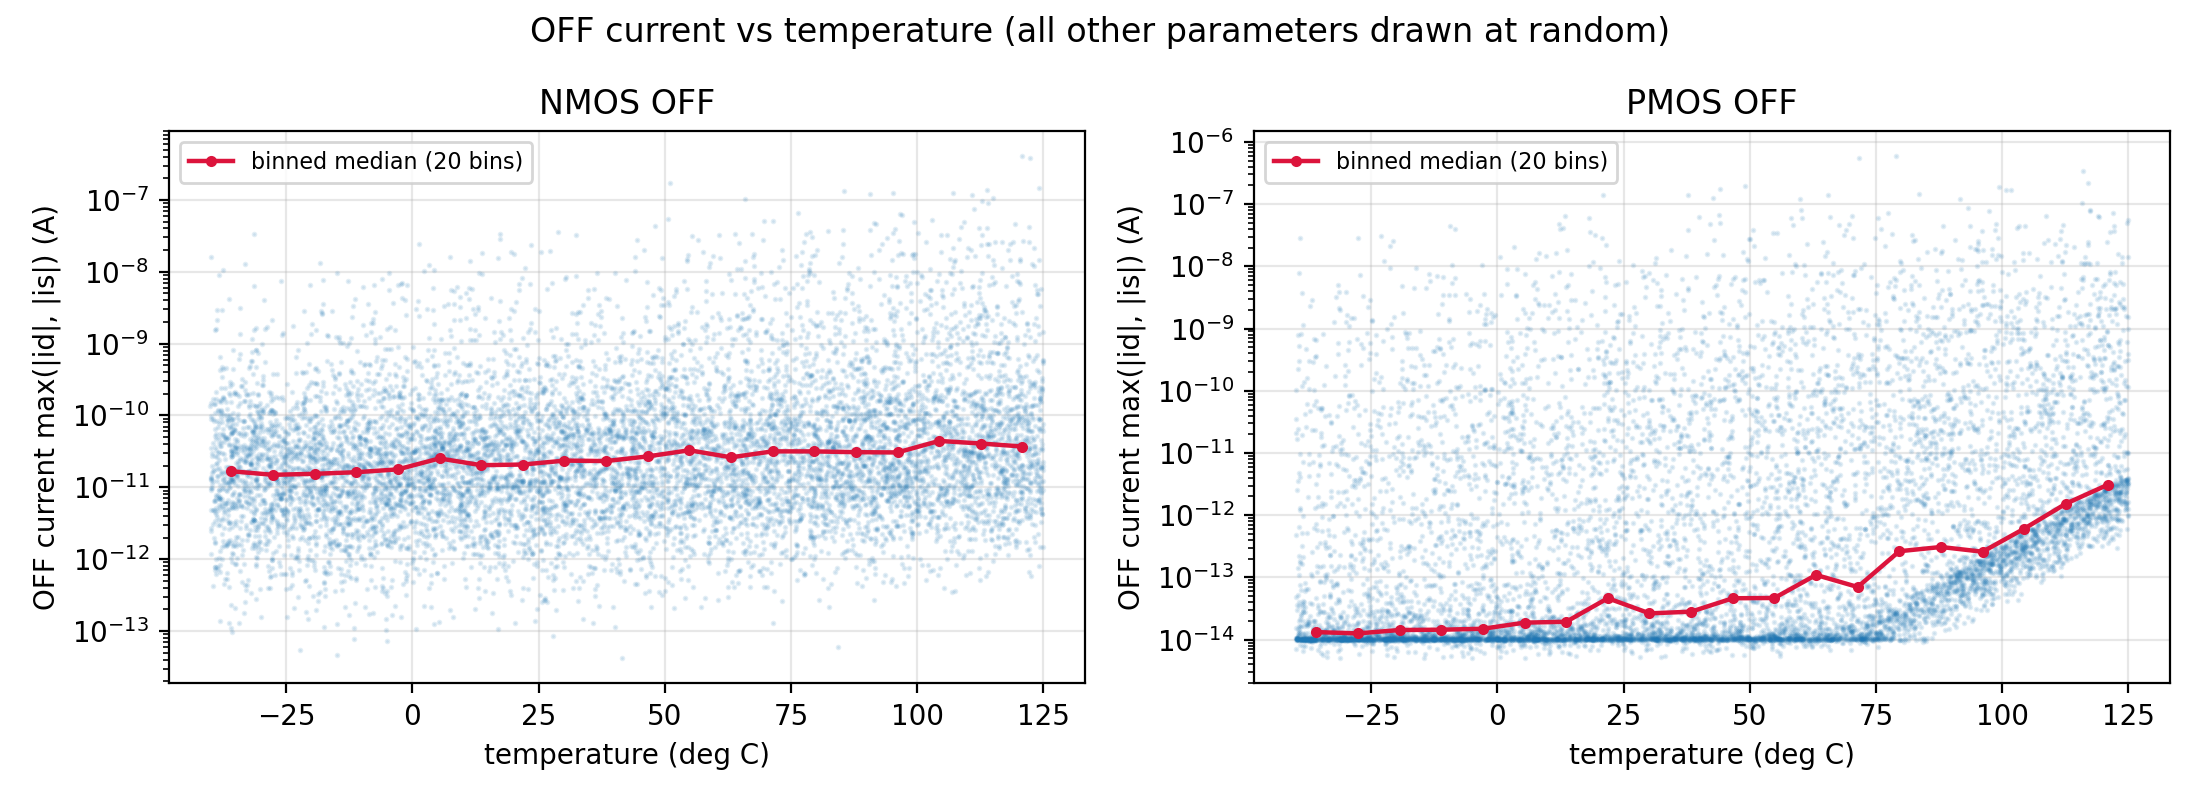
\includegraphics[width=0.49\textwidth]{figures/trend_off_vs_temperature.png}\hfill
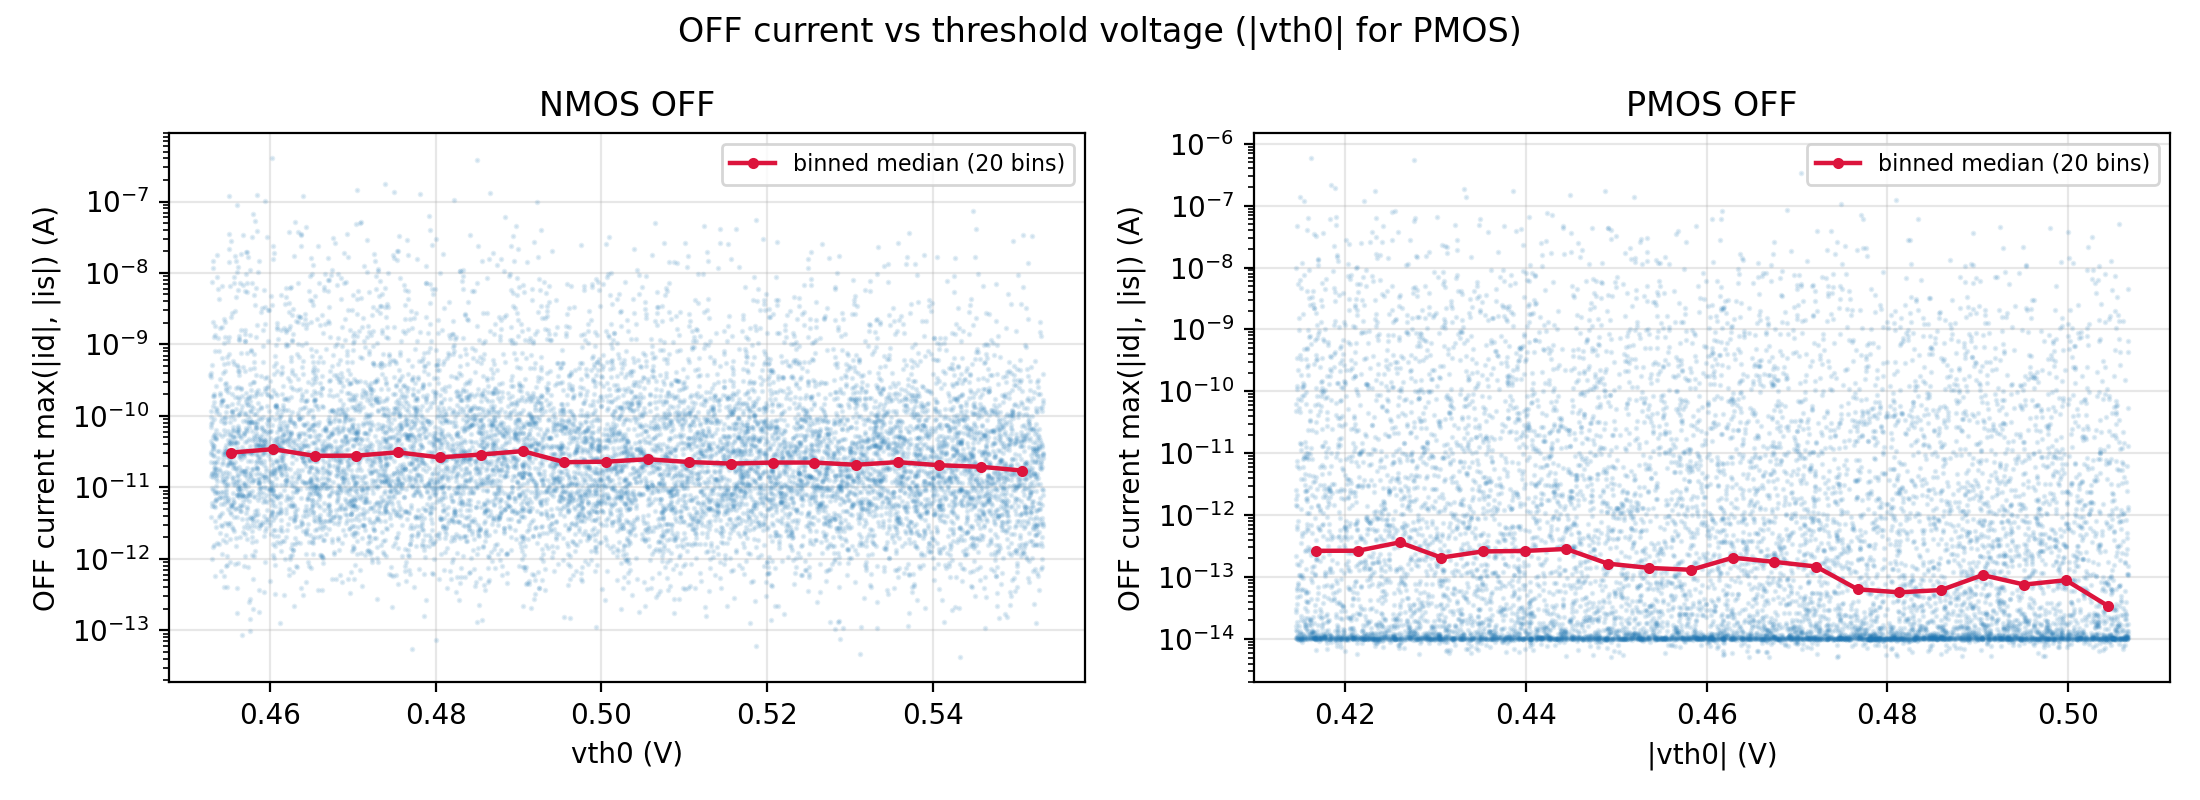
\includegraphics[width=0.49\textwidth]{figures/trend_off_vs_vth0.png}
\caption{OFF current $\max(|i_d|,|i_s|)$ versus temperature (left) and versus $|V_{th0}|$ (right) for NMOS OFF and PMOS OFF; faint points are the 10,000 samples, the red line is the median in 20 bins.}
\label{fig:trend1}
% src: partA_transistor/data_check/trend_off_vs_temperature.png, trend_off_vs_vth0.png
\end{figure*}
\begin{figure*}[t]
\centering
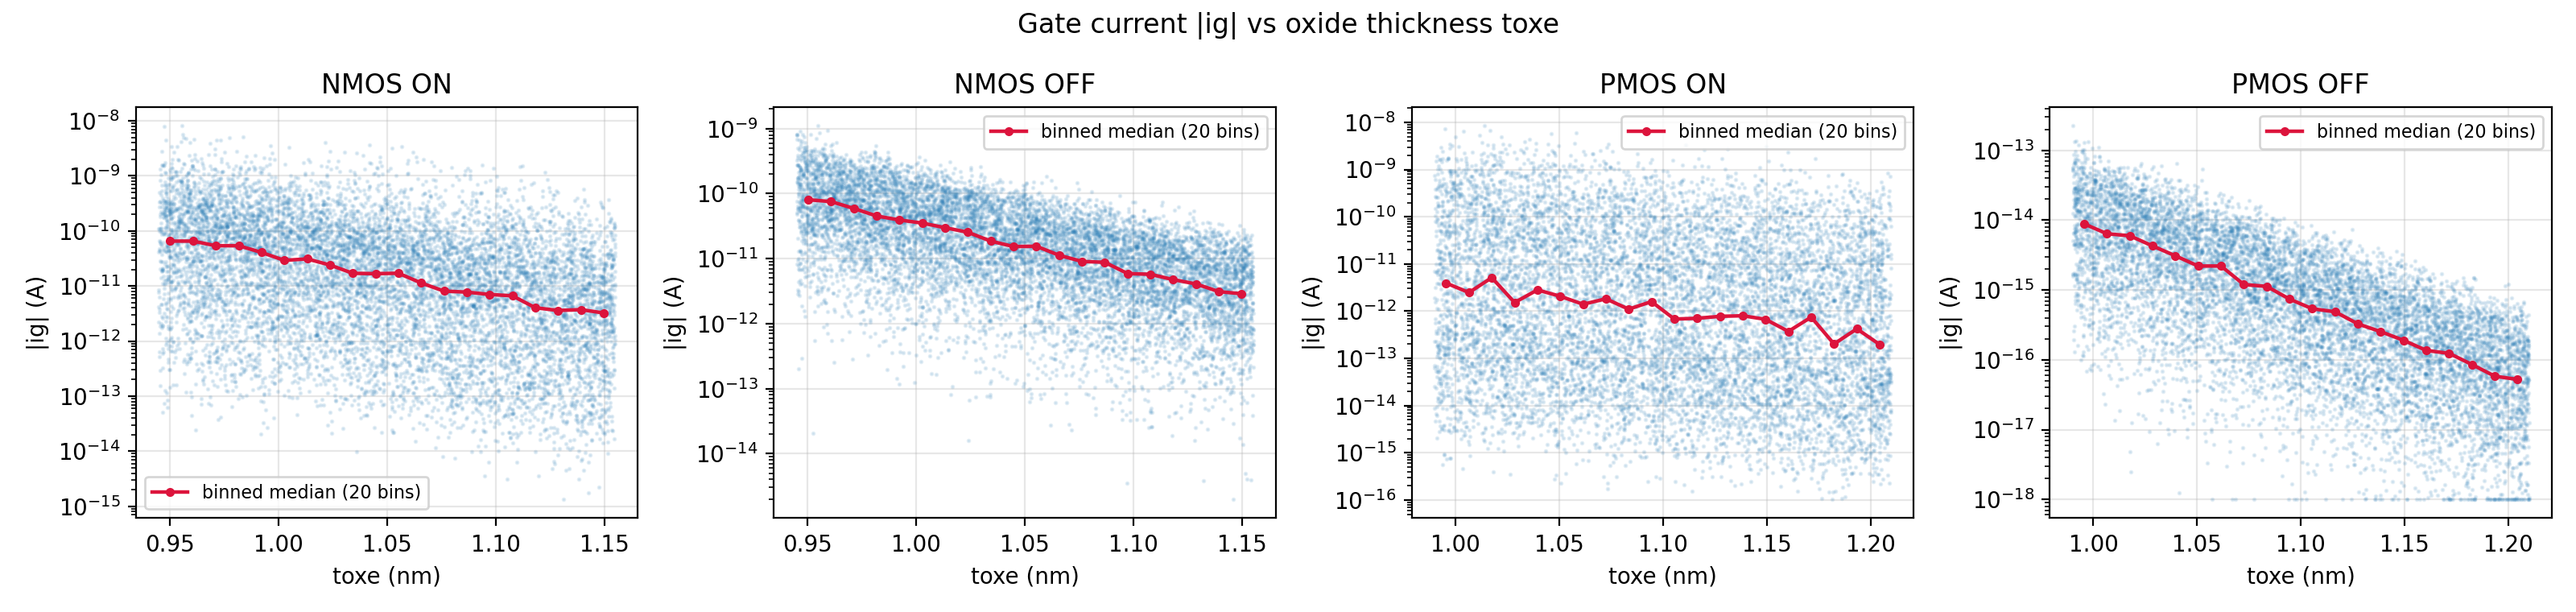
\includegraphics[width=0.9\textwidth]{figures/trend_ig_vs_toxe.png}
\caption{Gate current $|i_g|$ versus oxide thickness for all four cases (tunnelling current: steep fall of the median with toxe).}
\label{fig:trend2}
% src: partA_transistor/data_check/trend_ig_vs_toxe.png
\end{figure*}

\subsection{PMOS OFF gate and body currents}\label{sec:data:readout}
In ngspice a voltage-source branch current is rounded to steps of about \SI{2.22e-16}{\ampere}, while the PMOS OFF gate current is far smaller: 82.51\,\% of the rows have $|i_g|<\SI{5e-15}{\ampere}$. With $i_g=-i(V_g)$ the original PMOS OFF data were mostly rounding noise (1,760 exact zeros, 224 negative values and only 421 distinct values in 10,000 rows). The final netlist therefore reads $i_g$ and $i_b$ from the BSIM4 instance currents, $i_g=-(i_{gs}+i_{gd}+i_{gb}+i_{gcs}+i_{gcd})$ and $i_b=-(i_{bd}+i_{bs})+i_{gb}+i_{sub}+i_{gidl}+i_{gisl}$, which gives 9,977 distinct values and no zeros or negative values; where the source readout is resolvable it agrees to $\num{1.34e-3}$ relative or better. Every terminal still has its own voltage source.
% src: results/analysis/report_numbers/pmos_off_readout_precision.csv, report_data_stats.txt; partA_transistor/netlists/pmos_off_ngspice.cir

\subsection{Output precision, corners and sizing}\label{sec:data:corners}
\texttt{echo} prints six significant digits, so a stored value is rounded by at most $\num{5e-6}$ relative: negligible for currents, but a difference of two six-digit voltages near \SI{1}{\volt} is resolved only to about $10^{-5}$\,\si{\volt} (for NAND2 with inputs 00 the ON-PMOS $|V_{ds}|$ is exactly zero at the stored precision in 130 of 200 rows), which is why the gate leakage is built as in Sec.~\ref{sec:gates:method}.
A corner is one draw of $V_{DD}$, temperature and process parameters; all NMOS of a circuit share one draw and all PMOS another. The 200 corners of Parts~B and~C come from \texttt{rndseed=16} with an identical block and order in all six netlists, so corner~$k$ is the same everywhere (difference 0). Because the random stream behind \texttt{rndseed} depends on the ngspice build, the saved CSV files define the corners and all evaluation reads them.
Gates use $L=\SI{22}{\nano\meter}$ and widths of $2L_{min}$, $4L_{min}$ or $8L_{min}$ inside the training range: inverter PMOS \SI{88}{\nano\meter}, NMOS \SI{44}{\nano\meter}; NAND2 \SI{88}{\nano\meter}; NOR2 PMOS \SI{176}{\nano\meter} (series stack widened), NMOS \SI{44}{\nano\meter}; AND2 and OR2 are the NAND2/NOR2 followed by the inverter. The CLA uses the same gate subcircuits.
% src: validation_checks/digits_check.txt, results/analysis/report_numbers/on_pmos_vds_resolution.csv, validation_checks/b_consistency.txt, partB_gates/netlists/*.cir

\section{Data Check}\label{sec:datacheck}

\textbf{Kirchhoff check.} Because the currents are recorded into the terminals, $i_d+i_g+i_s+i_b$ must vanish. Table~\ref{tab:kcl} gives the residual for every case: the median is at most $\num{1.14e-6}$ of the largest terminal current (the six-digit CSV precision and \texttt{reltol}$=10^{-6}$; $\num{4.85e-9}$ for PMOS ON) and the 95th percentile is below $\num{5.6e-6}$ in all four cases. The only larger residuals are 15 NMOS ON and 18 PMOS ON rows with a relative residual above $10^{-3}$ (maximum $\num{2.84e-2}$ and $\num{1.36e-2}$); all are barely-on devices whose largest terminal current is at most $\SI{1.4e-13}{\ampere}$, with an absolute residual of at most $\SI{7.7e-16}{\ampere}$, about three times the $\num{2.2e-16}$\,A resolution of the branch-current readout.
% src: partA_transistor/data_check/kcl_check.csv, partA_transistor/data_check/README.md
\begin{table}[t]
\caption{Kirchhoff check of the four datasets (relative = divided by the largest terminal current of the row).}
\label{tab:kcl}
\centering\footnotesize
\setlength{\tabcolsep}{2.5pt}
\fitcol{% src: partA_transistor/data_check/kcl_check.csv
\begin{tabular}{lrrrrr}
\toprule
Case & Median $|\Sigma I|$ (A) & Max $|\Sigma I|$ (A) & Median rel. & P95 rel. & Max rel. \\
\midrule
NMOS ON & \num{8.18e-12} & \num{9.87e-10} & \num{5.1e-07} & \num{4.2e-06} & \num{2.8e-02} \\
NMOS OFF & \num{2.59e-17} & \num{8.29e-13} & \num{8.5e-07} & \num{3.9e-06} & \num{9.0e-06} \\
PMOS ON & \num{4.20e-14} & \num{1.00e-10} & \num{4.8e-09} & \num{1.6e-06} & \num{1.4e-02} \\
PMOS OFF & \num{1.00e-19} & \num{9.16e-13} & \num{1.1e-06} & \num{5.5e-06} & \num{9.9e-06} \\
\bottomrule
\end{tabular}
}
\end{table}

\textbf{Trend plots.} Figures~\ref{fig:trend1} and~\ref{fig:trend2} show the OFF current $\max(|i_d|,|i_s|)$ against temperature and against the threshold voltage, and the gate current $|i_g|$ against the oxide thickness, on log axes with the binned median. (Drain and source swap roles when $V_s>V_d$, so the larger of $|i_d|$ and $|i_s|$ is the channel leakage in either orientation.) All three trends have the expected sign in every case: the OFF current rises with temperature and falls with the threshold voltage, and the gate current falls steeply with the oxide thickness, by a factor of 20 to 170 over the 0.945--1.155\,nm range.
Over all rows the temperature and $V_{th}$ trends are diluted, because the OFF current also contains junction and gate-induced-drain leakage that depend little on either (a floor near $10^{-14}$\,A for PMOS OFF in Fig.~\ref{fig:trend1}). Restricting to the subthreshold regime (source within 50\,mV of its rail, other terminal more than 0.5\,V away, about 500 rows per case) gives the textbook behaviour: $+0.90$ (NMOS) and $+0.81$ (PMOS) decades per 100\,$^\circ$C and $-0.55$ and $-0.59$ decades per 50\,mV of $V_{th}$, i.e.\ roughly 84--91\,mV per decade.
% src: partA_transistor/data_check/trend_numbers.csv, partA_transistor/data_check/README.md
\begin{figure*}[t]
\centering
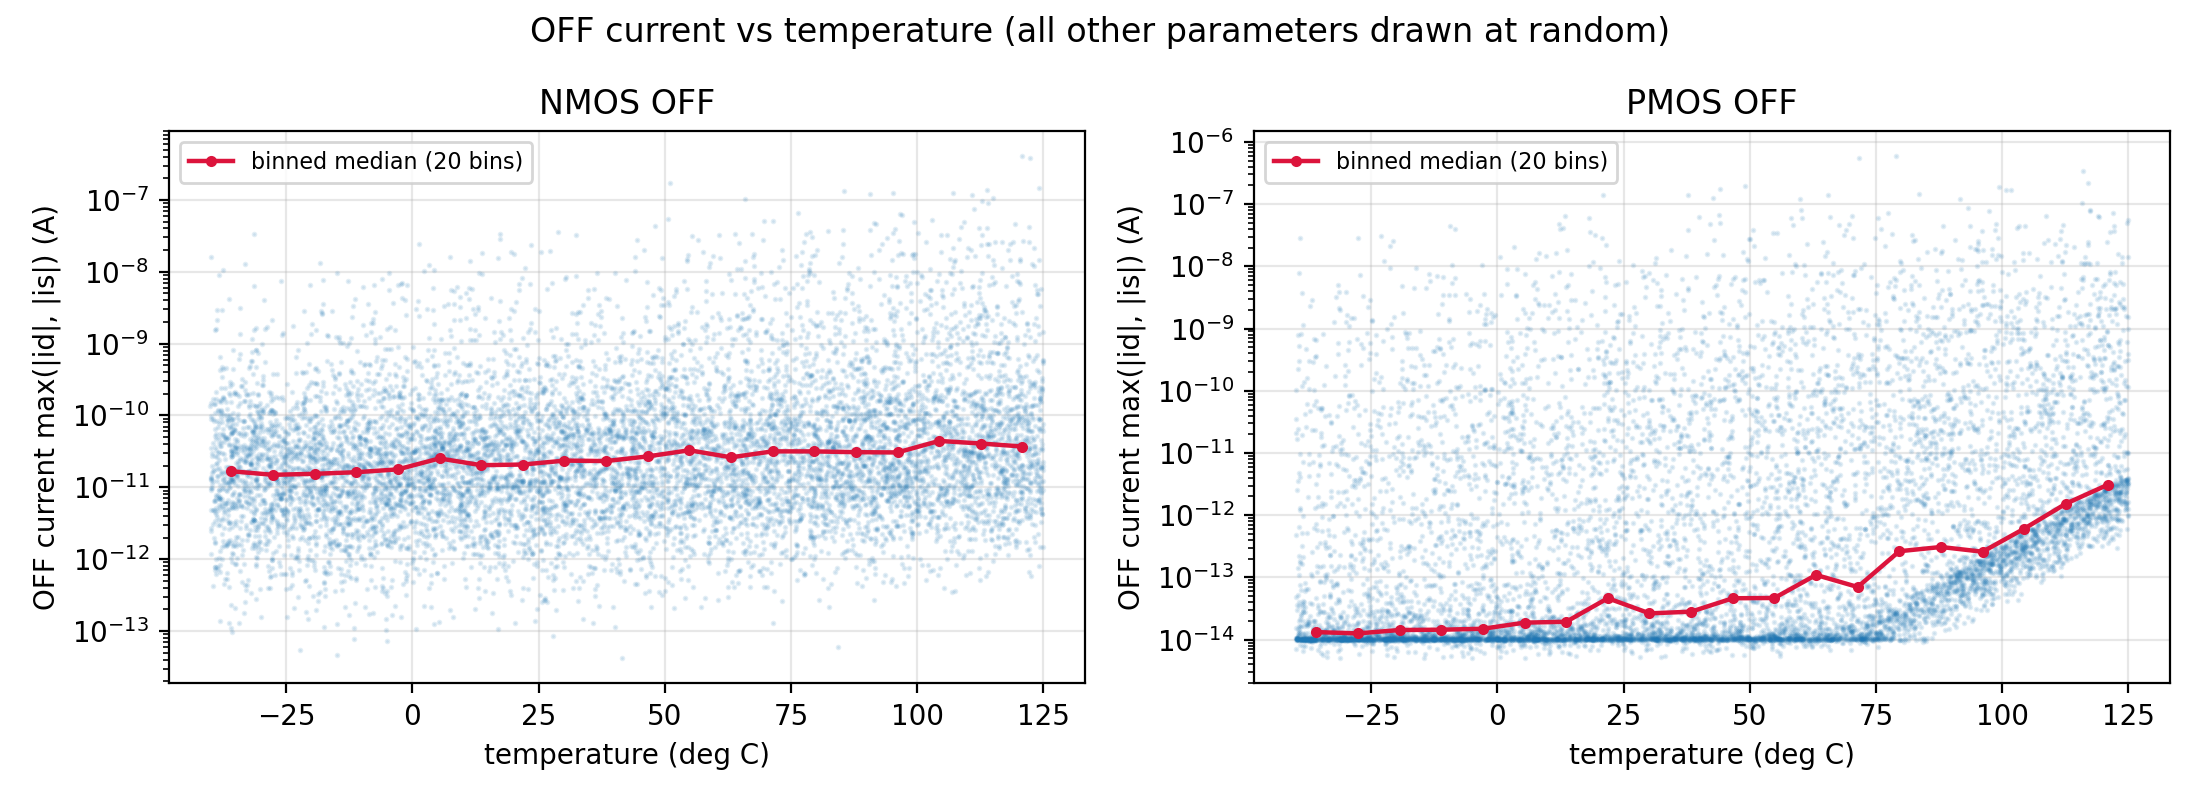
\includegraphics[width=0.49\textwidth]{figures/trend_off_vs_temperature.png}\hfill
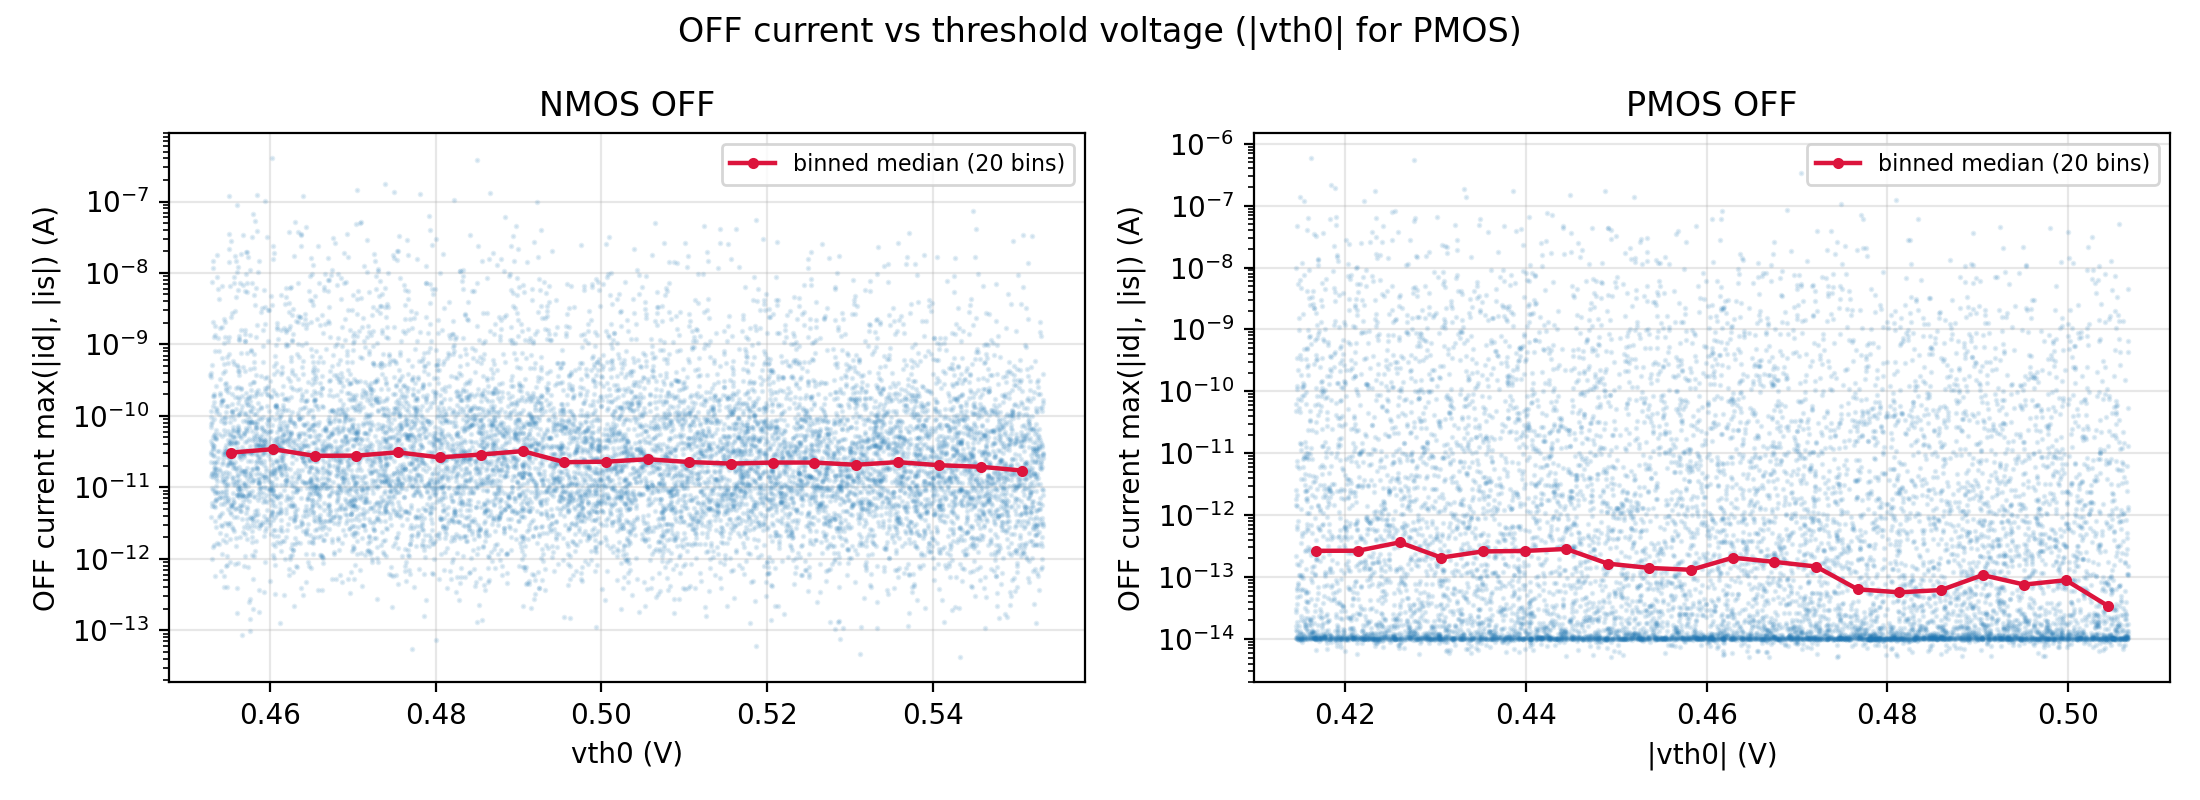
\includegraphics[width=0.49\textwidth]{figures/trend_off_vs_vth0.png}
\caption{OFF current $\max(|i_d|,|i_s|)$ versus temperature (left) and versus $|V_{th0}|$ (right) for NMOS OFF and PMOS OFF; faint points are the 10,000 samples, the red line is the median in 20 bins.}
\label{fig:trend1}
% src: partA_transistor/data_check/trend_off_vs_temperature.png, trend_off_vs_vth0.png
\end{figure*}
\begin{figure*}[t]
\centering
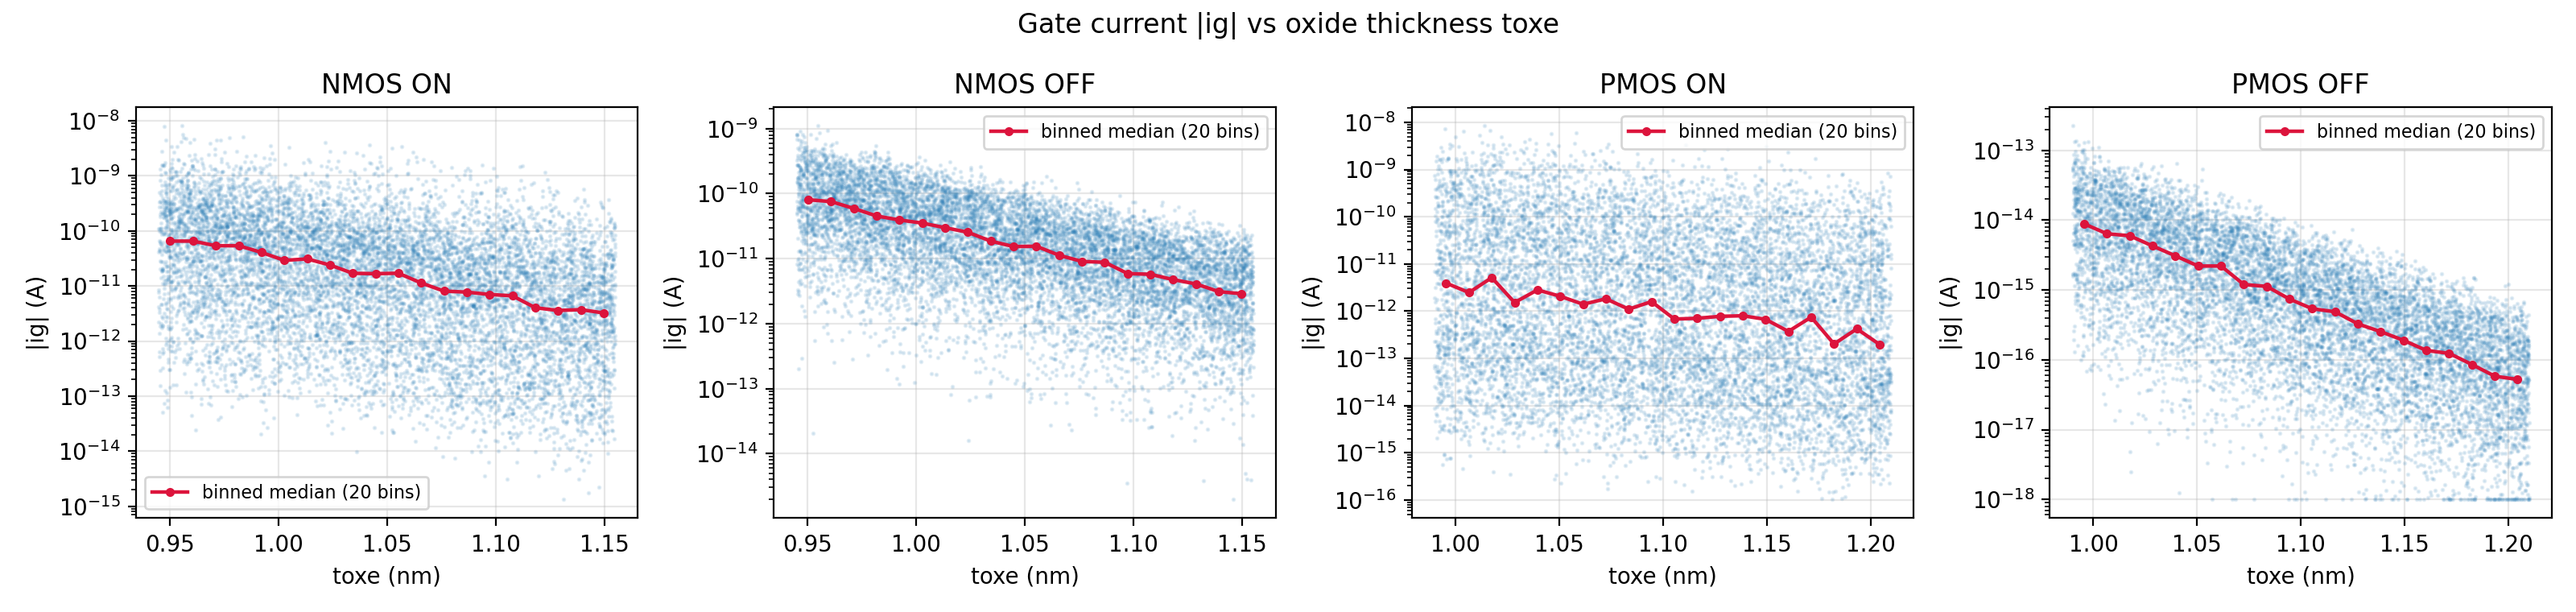
\includegraphics[width=0.9\textwidth]{figures/trend_ig_vs_toxe.png}
\caption{Gate current $|i_g|$ versus oxide thickness for all four cases (tunnelling current: steep fall of the median with toxe).}
\label{fig:trend2}
% src: partA_transistor/data_check/trend_ig_vs_toxe.png
\end{figure*}

\section{Transistor Models}\label{sec:models}

\subsection{Inputs, targets and signs}\label{sec:models:io}
The inputs are the ten varying quantities (vdd, temp, $W$, $V_d$, $V_s$, vth0, toxe, ndep, u0, xj; $V_g$ and $V_b$ are fixed by the case) plus ten physics features, standardised on the training split: $V_{ds}$, $|V_{ds}|$, the gate-source and body-source voltages relative to the \emph{effective source} (lower terminal for NMOS, higher for PMOS), $1/T$, the subthreshold term $(|V_{gs}|-|V_{th0}|)/V_T$, the oxide fields $|V_g-V_d|/t_{ox}$ and $|V_g-V_s|/t_{ox}$, $\log_{10}W$ and $\log_{10}(1-e^{-|V_{ds}|/V_T})$.
The target is $\log_{10}|I|$ of each terminal current (floor $10^{-18}$\,\si{\ampere} $=$ \texttt{abstol}), so the models span 12 decades. Signs are restored afterwards: in the ON cases $\operatorname{sign}(i_d)=\operatorname{sign}(V_d-V_s)$; in the OFF cases the effective drain has a fixed sign and the sign of the effective source current comes from a gradient-boosting classifier that also sees the KCL margin; $i_g$ and $i_b$ use a fixed sign or a classifier if their sign changes. The error of a prediction is the relative error $|{\hat I}-I|/|I|$, so a wrong sign costs at least 100\,\%.
% src: ml/pipeline.py (build_features, SignModel, relative_error_percent)

\subsection{Model types}\label{sec:models:types}
Four types are compared. All networks use the Huber loss ($\delta=0.05$ decades~\cite{huber}) on the standardised target, AdamW~\cite{adamw} (learning rate $10^{-3}$, weight decay $10^{-4}$), a cosine schedule, batch size 128, 500 epochs, and keep the epoch with the lowest validation loss.
\textbf{ResNet MLP}~\cite{resnet}: Linear(20$\rightarrow$256), residual blocks $h\leftarrow h+W_2\,\mathrm{SiLU}(W_1\,\mathrm{SiLU}(h))$ (3 blocks by default), one network per output group ($i_d$ and $i_s$ together, $i_g$, $i_b$).
\textbf{Hybrid}: a closed-form compact model (EKV channel current~\cite{ekv} with DIBL and body effect, gate tunnelling, reverse junction leakage, GIDL; 31 fitted constants for NMOS ON) fitted to $\log_{10}|I|$ by least squares~\cite{scipy}, plus a 256-128-64 SiLU MLP per group for the residual.
\textbf{GPR}~\cite{rasmussen}: an exact Gaussian process per current with an ARD RBF or Mat\'ern-5/2 kernel chosen on the validation MAE; hyper-parameters by marginal likelihood on 2,000 random training rows (Adam~\cite{adam}, 300 steps, float64), then conditioned on all 8,000 rows.
\textbf{PINN}~\cite{pinn}: a 256-128-64 SiLU MLP per group with the Huber loss plus a Kirchhoff penalty on the signed currents, a monotonicity penalty (derivatives with respect to $W$, toxe, $|V_{th0}|$ and $T$ of verified sign) and an EKV channel-current prior; five physics variants are trained and the best per group on validation is kept.
% src: ml/models.py, results/analysis/report_numbers/model_facts.txt

\ifexpFirstModels
\subsection{Earlier model set, benchmark and the components model}\label{sec:models:first}
Before fixing the final types, 29 regression model types were benchmarked on a first split (70:15:15, seed 42) with identical features, targets and metrics.
In that set a components MLP was the best OFF model, but it learns from the BSIM4 \emph{internal} component currents, which are not among the 16 dataset columns, so it is excluded and the physics-informed network is the fourth type.
The compliant models still give better gate- and circuit-level results: with GPR for ON and ResNet for OFF the first set reaches 98.58\,\% (gates) and 98.80\,\% (circuit), against 96.86\,\% and 96.27\,\% with the components MLP for OFF.
% src: archive/model_benchmark/results/summary_validation.csv, validation_checks/d1_validation_table.csv, results/phase2_comparison/comparison.csv
\fi

\subsection{Final models: 80:10:10 split and four compliant types}\label{sec:models:final}
The final set trains GPR, hybrid, ResNet and PINN on the four cases with an 80:10:10 split (8,000 / 1,000 / 1,000 rows, seed 42), using only the four dataset currents as targets. Per case, the type with the lowest mean validation median error over the four currents is chosen (the mean 95th percentile breaks ties); the test set is not used for any choice. Table~\ref{tab:modelcomp} compares the four types on the validation set, Table~\ref{tab:chosen} reports the chosen models on the test set, and the predicted-versus-SPICE plots are in Appendix~\ref{app:parity}.
Validation picks the hybrid model for NMOS ON, ResNet for NMOS OFF and PMOS OFF, and GPR for PMOS ON. For NMOS ON, hybrid, GPR and ResNet are tied (0.185, 0.186 and 0.186\,\% mean median error), so that choice is not significant. GPR is best where the physics is smooth (ON cases) and poor in the OFF cases (mean median error 1.37 and 2.12\,\%, 95th percentile above 22\,\%), where the current spans many decades and changes sign.
% src: results/partA/model_comparison_validation.csv, results/partA/chosen_models_test.csv
\textbf{Near-rail validation metric.} We added a second \emph{validation} metric, the mean error of $i_d$ and $i_s$ on the validation rows with $V_d$ and $V_s$ together within \SI{0.2}{\volt} of a rail, and tried a loss weight $w(r)=1+A\,e^{-r/\tau}$ ($\tau=\SI{50}{\milli\volt}$, $r$ the summed distance of $V_d$ and $V_s$ to the nearer rail). Rule, fixed beforehand: lowest near-rail error among weights whose normal validation score is within 10\,\% of the unweighted one. Validation chose $A=0$ (near-rail error 1.623\,\% against 1.684 and 1.824\,\% for $A=10$ and 30, whose normal scores of 0.533 and 0.523\,\% exceed the 10\,\% limit on the unweighted 0.353\,\%). The metric was added after the gate analysis, but all selection used validation data only.
% src: results/partA/rail_weight_tuning.csv, ml/choose_weight.py

\subsection{Tuning the ResNet for the OFF cases}\label{sec:models:tuning}
Most of the remaining gate error comes from the OFF transistors, so only the two ResNet OFF models were tuned: seven single changes of the defaults (3 blocks, width 256, 500 epochs, learning rate $10^{-3}$, batch 128, Huber $\delta=0.05$, weight decay $10^{-4}$), each trained on both OFF cases (Table~\ref{tab:tuning}). The rule was fixed before the runs: lowest near-rail validation error of $i_d$ and $i_s$ among settings whose normal validation score is at most 5\,\% worse than the default (limit 0.3705). Five residual blocks won (near-rail 1.162 against 1.623\,\%, score 0.326 against 0.353\,\%); width 512 and 1000 epochs gave a better score but a worse near-rail error, and a lower learning rate failed the limit. The tuning moved the Part~B mean accuracy from 98.89\,\% to 98.87\,\% and the Part~C accuracy from 98.89\,\% to 99.00\,\%.
% src: results/partA/resnet_tuning.csv, results/reference_before_tuning/evaluate_gates.log, evaluate_cla.log, results/partB/gate_predictions.csv, results/partC/cla3_results.csv
\begin{table}[t]
\caption{ResNet tuning for the OFF cases (validation). Score: mean median error (\%); near-rail: mean error of $i_d,i_s$ on near-rail validation rows (\%); the rule selects blocks=5.}
\label{tab:tuning}
\centering\footnotesize
\setlength{\tabcolsep}{4pt}
\fitcol{% src: results/partA/resnet_tuning.csv (limit 1.05 x default = 0.3705)
\begin{tabular}{lrrc}
\toprule
Setting & Val. score & Near-rail & Within limit \\
\midrule
default & 0.353 & 1.623 & yes \\
blocks=5 & 0.326 & 1.162 & yes \\
batch\_size=64 & 0.365 & 1.661 & yes \\
epochs=1000 & 0.288 & 1.391 & yes \\
huber\_beta=0.02 & 0.337 & 1.476 & yes \\
lr=5e-4 & 0.481 & 1.929 & no \\
width=512 & 0.301 & 1.266 & yes \\
weight\_decay=0 & 0.361 & 1.549 & yes \\
\bottomrule
\end{tabular}
}
\end{table}

\ifexpSymmetry
\subsection{Drain--source symmetry of the OFF devices}\label{sec:models:symmetry}
A MOSFET is symmetric under exchange of drain and source, which would allow a preprocessing that orders the terminals. In SPICE the ON devices are symmetric (mirror error at most 0.31\,\%) but the OFF devices are not: the dominant PMOS OFF current changed by up to 171\,\% in 15 random rows. Equal explicit junction geometry (\texttt{AD}=\texttt{AS}, \texttt{PD}=\texttt{PS}) or \texttt{geomod}$=0$ removes the asymmetry exactly, so the cause is the default junction geometry of an instance without \texttt{AD/AS/PD/PS}. It matters only for small currents; at gate operating points the device is symmetric to $\num{2.0e-5}$ (NMOS) and $\num{4.6e-5}$ (PMOS). All data share the same default geometry, so \emph{no symmetry preprocessing is used}.
% src: validation_checks/sym_cause.csv, validation_checks/sym_check.txt, validation_checks/sym_cause.txt
\fi

\section{Gate-Level Results (Part B)}\label{sec:gates}

\subsection{Method}\label{sec:gates:method}
The reference is the SPICE simulation of five static-CMOS gates (INV, NAND2, NOR2, AND2, OR2; AND2 and OR2 are simulated as complete gates, not as sums) for every input combination at the same 200 corners (18 cases $\times$ 200 $=$ 3,600 simulations), recording the leakage drawn from the supply $-i(V_{sup})$, the internal node voltages ($x$ between the series NMOS, $y$ between the series PMOS, and the first-stage output for AND2/OR2) and the output voltage.
% src: partB_gates/README.md, partB_gates/data/*.csv
Following step~4 of the project document, the terminal voltages $(V_d,V_g,V_s,V_b)$ of every transistor are taken from these \emph{recorded} SPICE node voltages (inputs at 0 or $V_{DD}$, NMOS bodies at 0, PMOS bodies at $V_{DD}$), together with the width and the corner's process parameters; the ML side does not solve the circuit. The ML internal-node columns of the prediction table are therefore copies of the recorded SPICE voltages. A transistor is ON if its gate is above $V_{DD}/2$ (NMOS) or below $V_{DD}/2$ (PMOS), and the model of that case predicts its four currents $\hat\imath_{m,t}$ (into terminal $t\in\{d,g,s,b\}$ of transistor $m$).
% src: ml/evaluate_gates.py, results/partB/gate_predictions.csv

\textbf{Gate leakage from the predicted currents.} The current drawn from $V_{DD}$ equals the sum of the currents into all terminals connected to the supply node, \emph{including} the nodes that an ON PMOS ties to it. Let $\mathcal S$ be the \emph{super-node}: $V_{DD}$ plus every node joined to $\mathcal S$ through the drain--source channel of an ON PMOS (iterated). With $n(m,t)$ the node of terminal $t$ of $m$ and $\mathcal M_{in}$ the transistors whose drain, source and body all lie in $\mathcal S$,
\begin{equation}
I_{leak}=\sum_{\substack{m\notin\mathcal M_{in}\\ t:\,n(m,t)\in\mathcal S}}\hat\imath_{m,t}\;+\sum_{\substack{m\in\mathcal M_{in}\\ n(m,g)\notin\mathcal S}}\bigl(-\hat\imath_{m,g}\bigr),
\label{eq:supernode}
\end{equation}
because for a transistor inside $\mathcal S$ Kirchhoff's law gives $i_d+i_s+i_b=-i_g$. The large channel current of an ON PMOS, which has almost no voltage across it, therefore cancels exactly and never has to be predicted (Fig.~\ref{fig:supernode}); what remains are OFF-transistor currents and gate currents.
\begin{figure}[t]
\centering
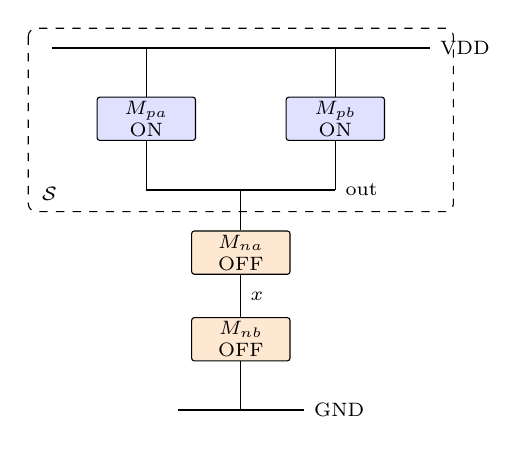
\begin{tikzpicture}[font=\scriptsize,
  tr/.style={draw,rounded corners=1pt,minimum width=1.25cm,minimum height=0.55cm,inner sep=1pt,align=center},
  on/.style={tr,fill=blue!12}, off/.style={tr,fill=orange!18}]
\draw[thick] (-2.4,2.7) -- (2.4,2.7) node[right]{VDD};
\node[on] (pa) at (-1.2,1.8) {$M_{pa}$\\ ON};
\node[on] (pb) at (1.2,1.8) {$M_{pb}$\\ ON};
\draw (pa.north) -- (-1.2,2.7); \draw (pb.north) -- (1.2,2.7);
\draw[thick] (-1.2,0.9) -- (1.2,0.9) node[right]{out};
\draw (pa.south) -- (-1.2,0.9); \draw (pb.south) -- (1.2,0.9);
\node[off] (na) at (0,0.1) {$M_{na}$\\ OFF};
\node[off] (nb) at (0,-1.0) {$M_{nb}$\\ OFF};
\draw (0,0.9) -- (na.north); \draw (na.south) -- (nb.north) node[midway,right]{$x$};
\draw[thick] (-0.8,-1.9) -- (0.8,-1.9) node[right]{GND}; \draw (nb.south) -- (0,-1.9);
\draw[dashed,rounded corners=3pt] (-2.7,2.95) rectangle (2.7,0.62);
\node[anchor=south west] at (-2.65,0.64) {$\mathcal S$};
\end{tikzpicture}
\caption{Super-node $\mathcal S$ (dashed) for a NAND2 with inputs 00. Both PMOS are ON, so $V_{DD}$ and the output form one node. The leakage of (\ref{eq:supernode}) is the current $\hat\imath_d$ of the OFF transistor $M_{na}$ leaving $\mathcal S$ plus $-\hat\imath_g$ of the two PMOS, whose drain, source and body all lie in $\mathcal S$; their channel currents cancel.}
\label{fig:supernode}
\end{figure}

\textbf{Metrics.} For every simulation $i$ the error is $e_i=(\hat I_i-I_i)/I_i$ with the ML leakage $\hat I_i$ and the SPICE leakage $I_i$; the bias is the median of $e_i$; a group is a gate case. The project document states a target of ``up to 99\,\% mean accuracy'' without defining it, so we use $A_1=1-\overline{|e|}$ as the headline and report three alternatives in Sec.~\ref{sec:assumptions}.

\subsection{Results}\label{sec:gates:results}
Over all 3,600 gate simulations the mean accuracy is 98.87\,\% (median 99.18\,\%, 95th percentile of $|e|$ 3.24\,\%, maximum 8.10\,\%); 35 rows exceed 5\,\% and 1,529 exceed 1\,\%. Per gate the mean accuracy is 98.47\,\% (INV), 99.02\,\% (NAND2), 98.96\,\% (NOR2), 98.84\,\% (AND2) and 98.85\,\% (OR2). The 18-case table is Table~\ref{tab:gate}, the parity plot Fig.~\ref{fig:gateparity}.
\textbf{The 99\,\% target is not reached at gate level:} 98.87\,\% is 0.13 points short. The most accurate cases are NAND2 \texttt{00} (99.49\,\%), NOR2 \texttt{11} (99.46\,\%) and NAND2 \texttt{10} (99.44\,\%); the least accurate are INV with input 0 (98.37\,\%), NOR2 \texttt{00} (98.38\,\%) and OR2 \texttt{11} (98.39\,\%). The latter three all contain an NMOS OFF transistor with the full supply across it; Sec.~\ref{sec:errors} traces the error to that operating point. The biases are small (between $-0.73$ and $+1.17\,\%$).
% src: results/partB/gate_predictions.csv, results/partB/gate_results.csv, results/analysis/report_numbers/error_breakdown.txt
\begin{table*}[t]
\caption{Gate results (final model set): SPICE and ML median leakage, bias (median signed error), median and 95th-percentile $|e|$, and mean accuracy $A_1$ for the 18 gate cases (200 corners each).}
\label{tab:gate}
\centering\footnotesize
% src: results/partB/gate_results.csv
\begin{tabular}{llrrrrrr}
\toprule
Gate & Inputs & SPICE med. (A) & ML med. (A) & Bias (\%) & Med. err. (\%) & P95 err. (\%) & Mean acc. (\%) \\
\midrule
INV & 0 & \num{2.19e-08} & \num{2.21e-08} & -0.73 & 1.24 & 4.35 & 98.37 \\
INV & 1 & \num{9.82e-08} & \num{9.81e-08} & +1.17 & 1.20 & 3.50 & 98.58 \\
\midrule
NAND2 & 00 & \num{5.40e-10} & \num{5.37e-10} & -0.03 & 0.39 & 1.29 & 99.49 \\
NAND2 & 01 & \num{5.00e-08} & \num{5.03e-08} & -0.13 & 1.09 & 4.29 & 98.57 \\
NAND2 & 10 & \num{8.53e-09} & \num{8.54e-09} & -0.08 & 0.34 & 1.83 & 99.44 \\
NAND2 & 11 & \num{1.95e-07} & \num{1.95e-07} & +1.14 & 1.19 & 3.48 & 98.59 \\
\midrule
NOR2 & 00 & \num{4.38e-08} & \num{4.42e-08} & -0.73 & 1.24 & 4.34 & 98.38 \\
NOR2 & 01 & \num{2.04e-07} & \num{2.02e-07} & +0.69 & 0.96 & 3.50 & 98.79 \\
NOR2 & 10 & \num{1.61e-08} & \num{1.61e-08} & +0.44 & 0.64 & 1.98 & 99.23 \\
NOR2 & 11 & \num{2.26e-10} & \num{2.28e-10} & -0.12 & 0.42 & 1.42 & 99.46 \\
\midrule
AND2 & 00 & \num{9.92e-08} & \num{9.98e-08} & +1.16 & 1.19 & 3.48 & 98.59 \\
AND2 & 01 & \num{1.67e-07} & \num{1.66e-07} & +0.06 & 0.82 & 2.74 & 99.05 \\
AND2 & 10 & \num{1.13e-07} & \num{1.14e-07} & +0.80 & 0.91 & 3.27 & 98.77 \\
AND2 & 11 & \num{2.26e-07} & \num{2.30e-07} & +0.46 & 0.78 & 2.88 & 98.95 \\
\midrule
OR2 & 00 & \num{1.60e-07} & \num{1.61e-07} & +0.03 & 0.80 & 2.74 & 99.01 \\
OR2 & 01 & \num{2.38e-07} & \num{2.41e-07} & +0.08 & 0.81 & 2.88 & 98.99 \\
OR2 & 10 & \num{4.31e-08} & \num{4.22e-08} & -0.39 & 0.74 & 2.75 & 99.02 \\
OR2 & 11 & \num{2.22e-08} & \num{2.23e-08} & -0.72 & 1.20 & 4.34 & 98.39 \\
\bottomrule
\end{tabular}

\end{table*}
\begin{figure}[t]
\centering
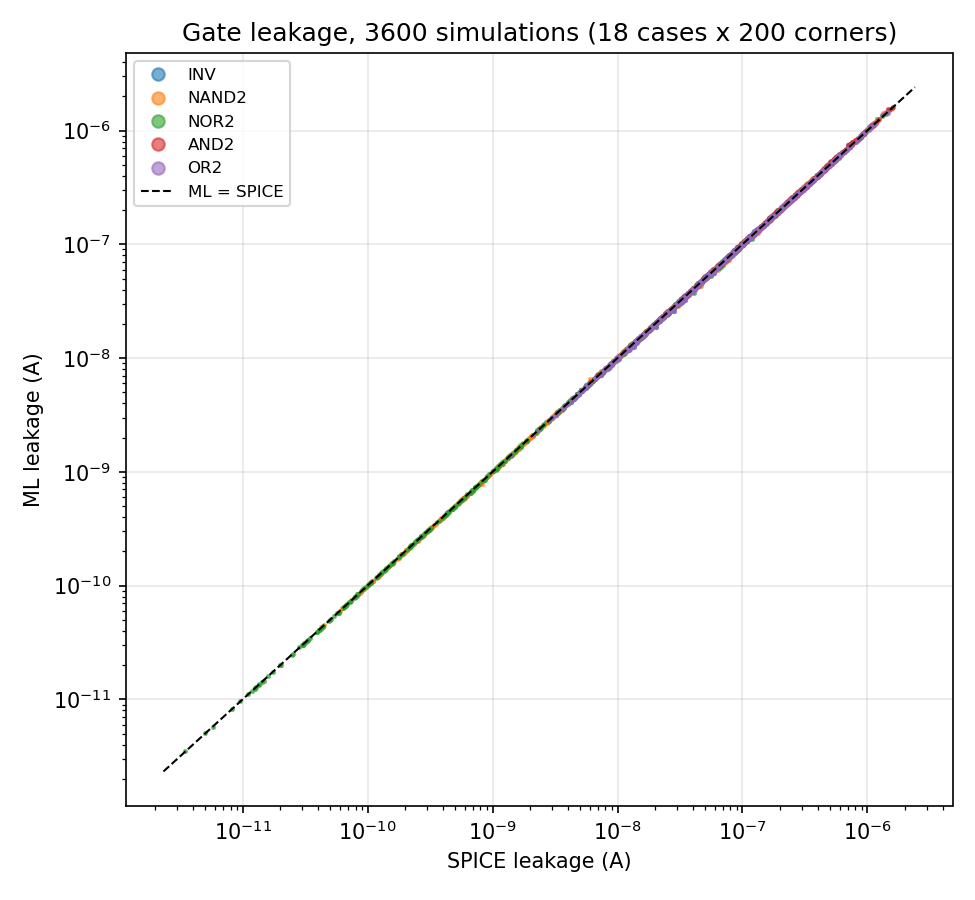
\includegraphics[width=\columnwidth]{figures/gate_parity.png}
\caption{ML versus SPICE leakage for all 3,600 gate simulations (log axes, dashed line: ML $=$ SPICE). The points follow the diagonal over about five decades; the deviations are at the percent level (maximum 8.10\,\%).}
\label{fig:gateparity}
% src: results/partB/gate_parity.png
\end{figure}

\subsection{Why the plain current sum fails}\label{sec:gates:plain}
The literal reading of ``use the predicted currents to calculate the gate leakage'' is the sum of the predicted currents into the terminals tied to the $V_{DD}$ node. This fails by orders of magnitude (Table~\ref{tab:plainsum}): NAND2 and AND2 reach a mean accuracy of $-5.7\times10^{5}\,\%$ and $-2.2\times10^{3}\,\%$ with 265 rows of negative predicted leakage, and over all gates the mean accuracy is of the order of $-10^{5}\,\%$. The reason is the one of Sec.~\ref{sec:data:corners}: an ON PMOS inside a gate has almost no voltage across it, so its channel current is the small difference of two large numbers that the models cannot resolve, whereas (\ref{eq:supernode}) cancels it exactly.
\textbf{Check with exact currents.} We re-simulated 10 rows of every one of the 18 gate cases with a 0\,V source in series with every transistor terminal and fed the \emph{exact SPICE} terminal currents to (\ref{eq:supernode}) (same code as the ML evaluation, same ON/OFF rule): over 179 converged simulations the result reproduces the recorded leakage to $\num{8.0e-6}$ relative at worst (median $\num{6.5e-7}$), which is the six-digit CSV precision. The construction is therefore exact; all remaining gate error is model error.
% src: results/analysis/report_numbers/plain_sum_check.csv, validation_checks/c1_kcl_method.csv, c1_kcl_method.txt
\begin{table}[t]
\caption{Plain sum of the currents into the $V_{DD}$ terminals versus the super-node method (final models, 3,600 rows).}
\label{tab:plainsum}
\centering\footnotesize
\setlength{\tabcolsep}{2.5pt}
\fitcol{% src: results/analysis/report_numbers/plain_sum_check.csv
\begin{tabular}{lrrrrr}
\toprule
Gate & Plain sum: mean acc. (\%) & Neg. rows & Med. err. (\%) & Super-node: mean acc. (\%) & Med. err. (\%) \\
\midrule
INV & 16.7 & 0 & 3.43 & 98.47 & 1.23 \\
NAND2 & -567,002 & 137 & 41.13 & 99.02 & 0.58 \\
NOR2 & 56.1 & 0 & 1.74 & 98.96 & 0.74 \\
AND2 & -2,167 & 128 & 11.49 & 98.84 & 0.91 \\
OR2 & 24 & 0 & 23.00 & 98.85 & 0.86 \\
\midrule
All gates & -126,462 & 265 & 12.97 & 98.87 & 0.82 \\
\bottomrule
\end{tabular}
}
\end{table}

\section{Test-Circuit Results (Part C)}\label{sec:circuit}

\subsection{Method}\label{sec:circuit:method}
The adder is built only from the gates of Part~B (27 NAND2, 3 INV, 2 AND2, 1 OR2). For every one of the 64 input vectors the logic value at the inputs of every gate is computed by evaluating the gates in topological order; the computed sum bits and carry-out equal the correct 3-bit sum for all 64 vectors and agree with the SPICE output voltages (threshold $V_{DD}/2$) in all 12,800 simulations.
For each vector and corner $k$, every gate's ML leakage is looked up from the Part~B prediction table by (gate type, input bits, corner), and the circuit leakage is the plain sum
\begin{equation}
\hat I_{CLA}(v,k)=\sum_{g=1}^{33}\hat I_{g}\bigl(\text{type}_g,\ \text{inputs}_g(v),\ k\bigr),
\label{eq:cla}
\end{equation}
which assumes that every gate input sits at exactly 0 or $V_{DD}$ and ignores loading between gates, as the project document prescribes. The reference is the SPICE simulation of the complete transistor netlist (64 vectors $\times$ 200 corners $=$ 12,800 rows, corners identical to Part~B).
As a diagnostic we also compute the \emph{ceiling}: the same sum with the Part~B \emph{SPICE} gate leakages instead of the ML ones, i.e.\ with perfect gate models. It isolates what the summation itself costs.
% src: ml/evaluate_cla.py, results/partC/cla3_gates.csv, results/partC/cla3_predictions.csv

\subsection{Results}\label{sec:circuit:results}
The plain sum of the ML gate leakages predicts the circuit leakage with a mean accuracy of 99.00\,\% (median 99.17\,\%), a bias of $-0.23\,\%$, a 95th percentile of $|e|$ of 2.57\,\% and a maximum of 4.02\,\% over 12,800 simulations (Table~\ref{tab:cla}, Fig.~\ref{fig:claparity}). The per-vector accuracy lies between 98.95\,\% (vector $3+3$) and 99.05\,\% (vector $0+7$), the median $|e|$ between 0.77 and 0.89\,\%, and the median SPICE leakage per vector between $\SI{2.72e-6}{\ampere}$ and $\SI{3.56e-6}{\ampere}$; the per-vector table is provided in the project repository. The worst row is vector $1+7$ at corner 39 (\SI{122}{\celsius}), $+4.02\,\%$; no row exceeds 5\,\%, 5,172 of 12,800 exceed 1\,\%.
\textbf{The margin to the 99\,\% target is small.} The ceiling is 99.16\,\%: even with perfect gate models the sum of isolated gate leakages underestimates the circuit leakage by 0.66\,\% (median) and cannot exceed 99.16\,\% mean accuracy. The ML result of 99.00\,\% sits just below this ceiling because the ML gate errors have a small \emph{positive} bias that offsets the negative summation bias: the ML sum exceeds the ceiling sum by a median of $+0.70\,\%$ (mean $+0.81\,\%$), so the circuit bias is $-0.23\,\%$ against $-0.66\,\%$ for the ceiling; Part~C is not better than Part~B because the models are better there, but because the two errors partly cancel. The project document expects the circuit accuracy to be lower than the gate accuracy because of the neglected loading; here it is not (99.00\,\% against 98.87\,\%) for exactly this reason.
% src: results/partC/cla3_results.csv, results/partC/cla3_predictions.csv, results/analysis/report_numbers/error_breakdown_partC.csv, results/analysis/loading_analysis/cancellation_check.txt
\begin{table}[t]
\caption{3-bit CLA, final models: ML (sum of the ML gate leakages) and ceiling (sum of the SPICE gate leakages), 12,800 simulations.}
\label{tab:cla}
\centering\footnotesize
\setlength{\tabcolsep}{3pt}
\fitcol{% src: results/partC/cla3_results.csv (row ALL)
\begin{tabular}{lrr}
\toprule
Metric & ML (sum of ML gates) & Ceiling (sum of SPICE gates) \\
\midrule
SPICE median (A) & \num{2.99e-06} & \num{2.99e-06} \\
Estimate median (A) & \num{3.01e-06} & \num{2.97e-06} \\
Bias (\%) & -0.23 & -0.66 \\
Median $|e|$ (\%) & 0.83 & 0.66 \\
P95 $|e|$ (\%) & 2.57 & 2.11 \\
Max $|e|$ (\%) & 4.02 & 3.83 \\
\midrule
Mean accuracy (\%) & 99.00 & 99.16 \\
Median accuracy (\%) & 99.17 & 99.34 \\
\bottomrule
\end{tabular}
}
\end{table}
% Table IX (Sec. VII-C, VIII-A), placed here so that the two-column float reaches the page of its first reference
\begin{table*}[t]
\caption{Mean $|e|$ (\%) by corner condition: Part~B (ML) and Part~C (ML and ceiling), and the median signed error (bias) of Part~C. Temperature ranges in $^\circ$C, quartiles of the NMOS $V_{th0}$ and the PMOS $|V_{th0}|$, terciles of $V_{DD}$.}
\label{tab:breakdown}
\centering\footnotesize
% src: results/analysis/report_numbers/error_breakdown_partB.csv, error_breakdown_partC.csv
\begin{tabular}{llrrrrr}
\toprule
Variable & Range & B: mean $|e|$ & C: mean $|e|$ ML & C: ceiling & C: bias ML & C: bias ceil. \\
\midrule
temperature & -40--0.0 & 1.50 & 1.16 & 0.56 & +0.26 & -0.40 \\
 & 0.0--40.0 & 1.14 & 0.99 & 0.48 & +0.44 & -0.37 \\
 & 40.0--85.0 & 0.98 & 1.03 & 0.89 & -0.54 & -0.78 \\
 & 85.0--125.0 & 0.92 & 0.83 & 1.38 & -0.56 & -1.22 \\
\midrule
NMOS vth0 quartile & Q1 (lowest) & 1.34 & 1.19 & 1.20 & -0.90 & -1.04 \\
 & Q2 & 1.12 & 0.90 & 0.98 & -0.51 & -0.90 \\
 & Q3 & 0.98 & 0.91 & 0.72 & -0.11 & -0.54 \\
 & Q4 (highest) & 1.08 & 0.99 & 0.46 & +0.63 & -0.34 \\
\midrule
PMOS $|$vth0$|$ quartile & Q1 (lowest) & 1.25 & 1.22 & 0.74 & +0.05 & -0.58 \\
 & Q2 & 1.09 & 0.99 & 0.92 & -0.19 & -0.76 \\
 & Q3 & 1.16 & 0.94 & 0.89 & +0.04 & -0.72 \\
 & Q4 (highest) & 1.02 & 0.84 & 0.81 & -0.48 & -0.72 \\
\midrule
VDD tercile & low VDD & 0.84 & 0.82 & 0.70 & -0.46 & -0.55 \\
 & mid VDD & 1.00 & 0.98 & 0.80 & -0.20 & -0.65 \\
 & high VDD & 1.55 & 1.20 & 1.01 & +0.31 & -0.82 \\
\bottomrule
\end{tabular}

\end{table*}
\begin{figure}[t]
\centering
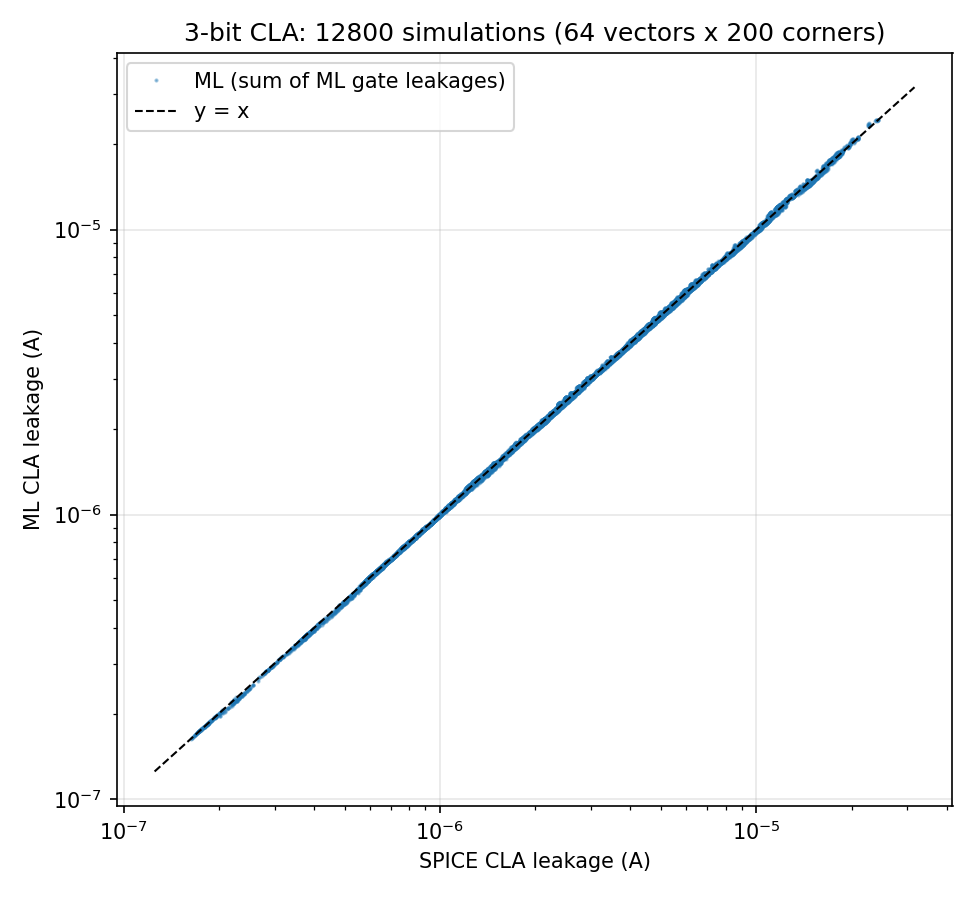
\includegraphics[width=\columnwidth]{figures/cla3_parity.png}
\caption{ML versus SPICE leakage of the 3-bit CLA for all 12,800 simulations (log axes, dashed line: ML $=$ SPICE).}
\label{fig:claparity}
% src: results/partC/cla3_parity.png
\end{figure}

\subsection{What limits the summation (ceiling analysis)}\label{sec:circuit:ceiling}
The ceiling error is not uniform: its mean $|e|$ grows from 0.56 and 0.48\,\% at $T\le40\,^\circ$C to 0.89 and 1.38\,\% at 40--85 and 85--125\,$^\circ$C, and its bias from $-0.40\,\%$ to $-1.22\,\%$ (Table~\ref{tab:breakdown}). The ML error does the opposite (1.16, 0.99, 1.03 and 0.83\,\%, bias $+0.26$, $+0.44$, $-0.54$, $-0.56\,\%$), which is again the cancellation described above.
Two contributions to the summation error can be identified. (i)~\emph{Loading:} in the isolated gate simulations the inputs are ideal sources, which supply (inputs at logic 1) or absorb (inputs at 0) a small gate current; in the circuit these currents flow through the driving gates. Adding the SPICE pin current of every input that is driven by another gate and is at logic 1 to the sum raises the ceiling from 99.16\,\% to 99.37\,\% (median 99.34 to 99.61\,\%, bias $-0.66$ to $-0.39\,\%$), i.e.\ it explains 0.21 of the 0.84 points. (ii)~\emph{Inputs off the rails:} the gate inputs inside the adder are not exactly 0 or $V_{DD}$. Over the 230,400 recorded internal and output node voltages the median distance to the nearer rail is \SI{0.30}{\milli\volt}, the 95th percentile \SI{3.1}{\milli\volt} and the maximum \SI{10.7}{\milli\volt}; 25.08\,\% of the node voltages are more than \SI{1}{\milli\volt} from a rail, and the median distance is five times larger above \SI{85}{\celsius} (0.92 against \SI{0.18}{\milli\volt}). Because leakage depends exponentially on such offsets and the offsets grow with temperature, this is the most plausible origin of the temperature-dependent remainder; we did not isolate it separately.
These two effects are what the project document means by ``ignores loading between gates''; the headline number of this report does not include them.
% src: results/analysis/report_numbers/error_breakdown_partC.csv, results/analysis/loading_analysis/cla_ceiling_with_pins.csv, results/analysis/loading_analysis/offrail_nodes.txt

\section{Error Analysis}\label{sec:errors}

\subsection{Where the errors are}\label{sec:errors:where}
\textbf{By case.} At gate level the three least accurate cases (INV \texttt{0}, NOR2 \texttt{00}, OR2 \texttt{11}; 98.37--98.39\,\%) each contain an NMOS OFF transistor with the full supply across it and its source on the ground rail; the most accurate cases (NAND2 \texttt{00}, NOR2 \texttt{11}, NAND2 \texttt{10}; 99.44--99.49\,\%) are among the cases with the smallest leakage (Table~\ref{tab:gate}).
\textbf{By corner.} Table~\ref{tab:breakdown} shows the mean $|e|$ by temperature range, threshold-voltage quartile and supply tercile. At gate level the error is largest in the coldest range (1.50\,\% below 0\,$^\circ$C against 0.92\,\% above 85\,$^\circ$C), at high supply voltage (1.55\,\% in the upper third of $V_{DD}$ against 0.84\,\% in the lower third) and at low threshold voltage (NMOS $V_{th0}$ quartile 1: 1.34\,\% against 0.98\,\% in quartile 3; PMOS $|V_{th0}|$ quartile 1: 1.25\,\% against 1.02\,\% in quartile 4). The eight worst gate rows (7.1--8.1\,\%) are at corners 98 ($-11\,^\circ$C, $V_{DD}=\SI{1.06}{\volt}$, low PMOS $|V_{th0}|$), 151, 34 and 22. For the circuit the ML error does not grow with temperature (Sec.~\ref{sec:circuit:ceiling}); its worst rows are at corners 39 (122\,$^\circ$C, $V_{DD}=\SI{1.092}{\volt}$) and 192 (13\,$^\circ$C, $V_{DD}=\SI{1.062}{\volt}$), at most 4.02\,\%.
% src: results/analysis/report_numbers/error_breakdown_partB.csv, error_breakdown_partC.csv, error_breakdown.txt
\begin{table*}[t]
\caption{Mean $|e|$ (\%) by corner condition: Part~B (ML) and Part~C (ML and ceiling), and the median signed error (bias) of Part~C. Temperature ranges in $^\circ$C, quartiles of the NMOS $V_{th0}$ and the PMOS $|V_{th0}|$, terciles of $V_{DD}$.}
\label{tab:breakdown}
\centering\footnotesize
% src: results/analysis/report_numbers/error_breakdown_partB.csv, error_breakdown_partC.csv
\begin{tabular}{llrrrrr}
\toprule
Variable & Range & B: mean $|e|$ & C: mean $|e|$ ML & C: ceiling & C: bias ML & C: bias ceil. \\
\midrule
temperature & -40--0.0 & 1.50 & 1.16 & 0.56 & +0.26 & -0.40 \\
 & 0.0--40.0 & 1.14 & 0.99 & 0.48 & +0.44 & -0.37 \\
 & 40.0--85.0 & 0.98 & 1.03 & 0.89 & -0.54 & -0.78 \\
 & 85.0--125.0 & 0.92 & 0.83 & 1.38 & -0.56 & -1.22 \\
\midrule
NMOS vth0 quartile & Q1 (lowest) & 1.34 & 1.19 & 1.20 & -0.90 & -1.04 \\
 & Q2 & 1.12 & 0.90 & 0.98 & -0.51 & -0.90 \\
 & Q3 & 0.98 & 0.91 & 0.72 & -0.11 & -0.54 \\
 & Q4 (highest) & 1.08 & 0.99 & 0.46 & +0.63 & -0.34 \\
\midrule
PMOS $|$vth0$|$ quartile & Q1 (lowest) & 1.25 & 1.22 & 0.74 & +0.05 & -0.58 \\
 & Q2 & 1.09 & 0.99 & 0.92 & -0.19 & -0.76 \\
 & Q3 & 1.16 & 0.94 & 0.89 & +0.04 & -0.72 \\
 & Q4 (highest) & 1.02 & 0.84 & 0.81 & -0.48 & -0.72 \\
\midrule
VDD tercile & low VDD & 0.84 & 0.82 & 0.70 & -0.46 & -0.55 \\
 & mid VDD & 1.00 & 0.98 & 0.80 & -0.20 & -0.65 \\
 & high VDD & 1.55 & 1.20 & 1.01 & +0.31 & -0.82 \\
\bottomrule
\end{tabular}

\end{table*}

\subsection{Diagnosis: OFF transistors at the rails}\label{sec:errors:diag}
Why are these cases worse than the 0.3--0.6\,\% median error of the OFF models on the test split (Table~\ref{tab:chosen})? In a static gate every OFF transistor sits at a rail-to-rail operating point: for the inverter, input 0 gives NMOS OFF with $V_d\approx V_{DD}$ and $V_s=V_g=V_b=0$, input 1 gives PMOS OFF with $V_d\approx0$ and $V_s=V_g=V_b=V_{DD}$. The training data draw $V_d$ and $V_s$ uniformly, so this corner is sparse: only 76 (NMOS OFF) and 87 (PMOS OFF) of the 8,000 training rows have $|V_{ds}|>0.9\,V_{DD}$ (0.95 and 1.09\,\%), and only 27 and 26 rows (0.34 and 0.33\,\%) additionally have the source within 20\,mV of its rail. The project document fixes the uniform sampling, so we could not add samples there.
We re-simulated the inverter's OFF transistor alone (every terminal its own source, the 200 corners) and compared the final OFF models with it. The single-transistor dominant current reproduces the gate SPICE leakage (median relative difference $\num{2.0e-3}$ for NMOS, $\num{3.1e-7}$ for PMOS), so the gate evaluation setup is not the cause. At these operating points the median error of the dominant current is 1.24\,\% (NMOS) and 0.96\,\% (PMOS) with biases of $-0.73$ and $+0.79\,\%$, against test-split medians of 0.31\,\% ($i_d$) and 0.44\,\% ($i_d$) / 0.59\,\% ($i_s$): about four and two times larger. This matches the gate-level errors of Sec.~\ref{sec:gates:results} and is the main reason the gate accuracy is below 99\,\%. The near-rail validation metric of Sec.~\ref{sec:models:final} captures this region only partly: the five-block ResNet halves the NMOS OFF near-rail error (2.03 to 1.02\,\%) but PMOS OFF gets slightly worse (1.21 to 1.31\,\%), and the gate-level mean accuracy did not improve (98.89 to 98.87\,\%).
% src: results/analysis/report_numbers/rail_point_row_counts.csv, gate_point_replay_summary.csv, results/partA/chosen_models_test.csv, results/partA/resnet_tuning.csv, validation_checks/gate_point_replay.py

\section{Assumptions and Definitions}\label{sec:assumptions}
We state the following assumptions.

\textbf{1.\ Accuracy.} We define the accuracy of a set of simulations as $A_1=100\,\%-\overline{|e|}$ with the relative error $e=(\hat I-I)/I$ of each simulation, i.e.\ 100 minus the mean absolute percentage error. This is the strictest of the common readings and is the headline of this report. Table~\ref{tab:accdefs} gives the final models under three further definitions: 100 minus the median $|e|$, 100 minus the absolute mean signed error, and 100 minus the mean over groups (the 18 gate cases, or the 64 vectors) of $|\operatorname{med}(\hat I)/\operatorname{med}(I)-1|$. Only $A_1$ is below 99\,\% for Part~B; the signed-error definition rewards cancellation of errors of opposite sign and is not a measure of per-simulation accuracy.
% src: results/analysis/report_numbers/accuracy_definitions.csv
\begin{table}[t]
\caption{Final models under four accuracy definitions (\%).}
\label{tab:accdefs}
\centering\footnotesize
\setlength{\tabcolsep}{3pt}
\fitcol{% src: results/analysis/report_numbers/accuracy_definitions.csv
\begin{tabular}{lrrr}
\toprule
Definition (accuracy in \%) & Part B (ML) & Part C (ML) & Part C (ceiling) \\
\midrule
$100-\overline{|e|}$ & 98.87 & 99.00 & 99.16 \\
$100-\mathrm{median}|e|$ & 99.18 & 99.17 & 99.34 \\
$100-|\bar e|$ & 99.81 & 99.96 & 99.16 \\
$100-\overline{|\mathrm{med}_{\mathrm{ML}}/\mathrm{med}_{\mathrm{SPICE}}-1|}$ & 99.27 & 99.44 & 99.23 \\
\bottomrule
\end{tabular}
}
\end{table}

\textbf{2.\ Gate leakage.} The leakage of a gate is the current drawn from the $V_{DD}$ source, which is what the SPICE netlists record ($-i(V_{sup})$); the currents of the input sources are excluded. Their size relative to the recorded leakage is small except in two cases: for NOR2 with inputs \texttt{11}, the case with the smallest leakage of all (median $\SI{2.26e-10}{\ampere}$), the input sources supply a median of 56\,\% of the recorded leakage (maximum $6.6\times10^{3}\,\%$), and for NAND2 with inputs \texttt{00} they absorb a median of 45.8\,\% (maximum 98\,\%); for all other cases the median is below 1\,\%. With another definition the SPICE reference, and with it the gate-level accuracy, would change.
% src: results/analysis/loading_analysis/pin_current_shares.csv

\textbf{3.\ Training data.} The models are trained only on the 16 dataset columns of the project document (inputs: $V_{DD}$, temperature, $W$, terminal voltages, process parameters; targets: $i_d,i_g,i_s,i_b$). The components model of the first set, which learns from BSIM4 internal component currents that are not dataset columns, is therefore excluded from the final set (Sec.~\ref{sec:models:first}).

\textbf{4.\ PMOS OFF gate and body currents.} The PMOS OFF $i_g$ and $i_b$ are read from the BSIM4 instance currents because the source branch currents are rounded to about $\num{2.2e-16}$\,A, far above the true currents (Sec.~\ref{sec:data:readout}); every terminal still has its own voltage source.

\section{Limitations, Future Work and Conclusion}\label{sec:limits}
\textbf{Limitations.}
(i)~\emph{Sparse coverage of the gate operating points.} The remaining gate error comes from OFF transistors at rail-to-rail bias, where about 0.3\,\% of the training rows lie (Sec.~\ref{sec:errors:diag}); the project document fixes uniform sampling of $V_d,V_s$.
(ii)~\emph{The summation itself.} With perfect gate models the plain sum reaches only 99.16\,\% (Sec.~\ref{sec:circuit:ceiling}); about a quarter of the deficit comes from the input-pin currents and the rest, most plausibly, from gate inputs a few millivolts off the rails.
(iii)~\emph{Definitions.} Accuracy and gate leakage are defined by our assumptions (Sec.~\ref{sec:assumptions}).
(iv)~\emph{Single split, single seed.} All choices rest on one 80:10:10 split (seed 42) and one training seed; run-to-run standard deviations of the test median reach 0.40 for the ResNet, comparable to some of the differences used to choose between model types (e.g.\ the NMOS ON tie of 0.185, 0.186 and 0.186\,\%).
(v)~\emph{Data conventions.} PMOS OFF $i_g,i_b$ come from BSIM4 instance currents; six-digit CSV output limits what can be derived from node voltages; the corner stream depends on the ngspice build (Sec.~\ref{sec:data}).
(vi)~\emph{Scope.} Only DC operating points of fixed-size static gates and one adder in one technology are covered; no transient or loading effects.
% src: results/analysis/report_numbers/rail_point_row_counts.csv, results/partC/cla3_results.csv, results/analysis/loading_analysis/cla_ceiling_with_pins.csv, offrail_nodes.txt, archive/model_benchmark/seed_runs/summary_mean_std.csv

\textbf{Future work.} Within the specification the cheapest improvements are on the modelling side: more physics at the rails (a better analytical part of the hybrid model, features exposing the distance of the source to its rail), averaging several training seeds of the OFF ResNets, and a larger validation set to select by the near-rail error more reliably (it has only 90 near-rail rows per case). A learning curve (validation accuracy against training-set size) would show whether the OFF models are limited by data or by model form. Closing the summation gap needs the input-pin currents or predicted internal node voltages, i.e.\ a model beyond the four transistor models.

\textbf{Conclusion.} We built and checked a transistor $\rightarrow$ gate $\rightarrow$ circuit leakage estimator for the PTM \SI{22}{\nano\meter} HP technology. Four transistor models, one per case and chosen on a validation split from four model types, give test median errors of 0.03--0.59\,\% for the four terminal currents; assembled with Kirchhoff's current law on the supply node, they predict the leakage of five gates over 18 input cases and 200 PVT corners with a mean accuracy of 98.87\,\% (median 99.18\,\%) and, summed over 33 gates, the leakage of a 3-bit carry-lookahead adder over 64 vectors with a mean accuracy of 99.00\,\% (median 99.17\,\%). Against the 99\,\% target the gate level falls 0.13 points short and the circuit level meets it narrowly: the plain sum of isolated gate leakages caps the circuit accuracy at 99.16\,\% with perfect gate models, and the ML result benefits from a cancellation between the positive bias of the gate models and the negative bias of the summation. The remaining gate error is traced to OFF transistors at rail-to-rail bias, a corner that uniformly sampled training data cover with about 0.3\,\% of their rows.
% src: results/partA/chosen_models_test.csv (test medians 0.03--0.59), results/partB/gate_results.csv, results/partC/cla3_results.csv


\bibliographystyle{IEEEtran}
\bibliography{refs}

\appendices

\ifexpDist
\section{Distribution of the current magnitudes}\label{app:dist}
The leakage currents span many decades (Table~\ref{tab:dist}). The ON datasets are concentrated at $10^{-5}$--$10^{-4}$\,A (44.7\,\% of the NMOS ON and 46.7\,\% of the PMOS ON rows have $|i_s|$ in that decade). NMOS OFF is concentrated between $10^{-12}$ and $10^{-10}$\,A (67.7\,\% of the rows); PMOS OFF is spread almost evenly over the decades from below $10^{-15}$ to $10^{-11}$\,A (12--18\,\% per decade), and 63.5\,\% of its rows are below $10^{-12}$\,A.
Small currents inside the ON datasets come from weakly driven devices, not from the corner with both terminals at $V_{DD}$: of the 162 PMOS ON rows with $|i_d|$ between $10^{-13}$ and $10^{-11}$\,A, all have the higher of $V_d,V_s$ below $|V_{th0}|$ (subthreshold operation), none has both terminals within 100\,mV of $V_{DD}$, and only 99 of the 10,000 rows (0.99\,\%) have both terminals that close to $V_{DD}$.
% src: results/analysis/report_numbers/current_magnitude_distribution_pct.csv, report_data_stats.txt, validation_checks/pmos_on_small_currents2.txt
\begin{table}[t]
\caption{Distribution of $|i_s|$ in percent of the 10,000 rows per case.}
\label{tab:dist}
\centering\footnotesize
\setlength{\tabcolsep}{3pt}
\fitcol{% src: results/analysis/report_numbers/current_magnitude_distribution_pct.csv
\begin{tabular}{lrrrr}
\toprule
$|i_s|$ range (A) & NMOS ON & NMOS OFF & PMOS ON & PMOS OFF \\
\midrule
$<$1e-15 & 0.00 & 0.02 & 0.02 & 17.71 \\
1e-15--1e-14 & 0.01 & 0.11 & 0.06 & 15.94 \\
1e-14--1e-13 & 0.16 & 1.11 & 0.24 & 14.64 \\
1e-13--1e-12 & 0.34 & 9.52 & 0.59 & 15.23 \\
1e-12--1e-11 & 0.79 & 32.71 & 1.08 & 12.62 \\
1e-11--1e-10 & 1.60 & 35.03 & 1.96 & 9.90 \\
1e-10--1e-9 & 2.56 & 14.24 & 2.72 & 7.65 \\
1e-9--1e-8 & 3.58 & 5.67 & 3.62 & 4.55 \\
1e-8--1e-7 & 4.93 & 1.47 & 5.15 & 1.59 \\
1e-7--1e-6 & 7.37 & 0.12 & 8.33 & 0.17 \\
1e-6--1e-5 & 14.34 & 0.00 & 19.72 & 0.00 \\
1e-5--1e-4 & 44.66 & 0.00 & 46.69 & 0.00 \\
$>$=1e-4 & 19.66 & 0.00 & 9.82 & 0.00 \\
\bottomrule
\end{tabular}
}
\end{table}
\fi

\ifexpFamilies
\section{Gate accuracy per model family (for comparison only)}\label{app:family}
To see how much the model family matters at gate level we evaluated each family on its own for all four transistor cases (Table~\ref{tab:family}). \emph{These numbers are for comparison only; they were not used to choose the final models}, which were chosen on validation data only. The ResNet, which is among the best on the validation set, fails on NAND2 \texttt{00} (51.0\,\% mean accuracy with the 80:10:10 models, 24.6\,\% with the 70:15:15 models) because of its PMOS ON model: that case has the smallest leakage of the NAND2 cases (median $\SI{5.4e-10}{\ampere}$), and the gate currents of the two ON PMOS, which the super-node sum keeps, dominate it. GPR is accurate for the ON cases and is used there in the final set.
% src: results/analysis/report_numbers/family_gate_accuracy.csv, results/partB/gate_results.csv
\begin{table}[t]
\caption{One model family for all four cases, gate and circuit mean accuracy (\%); for comparison only, not used for selection.}
\label{tab:family}
\centering\footnotesize
\setlength{\tabcolsep}{2.5pt}
\fitcol{% src: results/analysis/report_numbers/family_gate_accuracy.csv
\begin{tabular}{llrrrr}
\toprule
Split & Family & Part B mean acc. & NAND2 00 & NAND2 all & Part C mean acc. \\
\midrule
80:10:10 & GPR & 94.48 & 96.15 & 94.93 & 93.19 \\
 & Hybrid & 96.96 & 79.78 & 93.77 & 97.60 \\
 & ResNet & 96.17 & 51.02 & 86.86 & 98.90 \\
 & PINN & 96.42 & 82.96 & 94.12 & 97.66 \\
\midrule
70:15:15 & GPR & 93.07 & 95.59 & 94.07 & 91.03 \\
 & Hybrid & 97.14 & 94.00 & 96.90 & 96.74 \\
 & ResNet & 94.39 & 24.64 & 79.98 & 98.81 \\
 & Components MLP & 95.47 & 74.95 & 91.69 & 96.27 \\
\bottomrule
\end{tabular}
}
\end{table}
\fi

\section{Predicted versus SPICE currents of the chosen models}\label{app:parity}
\begin{figure*}[t]
\centering
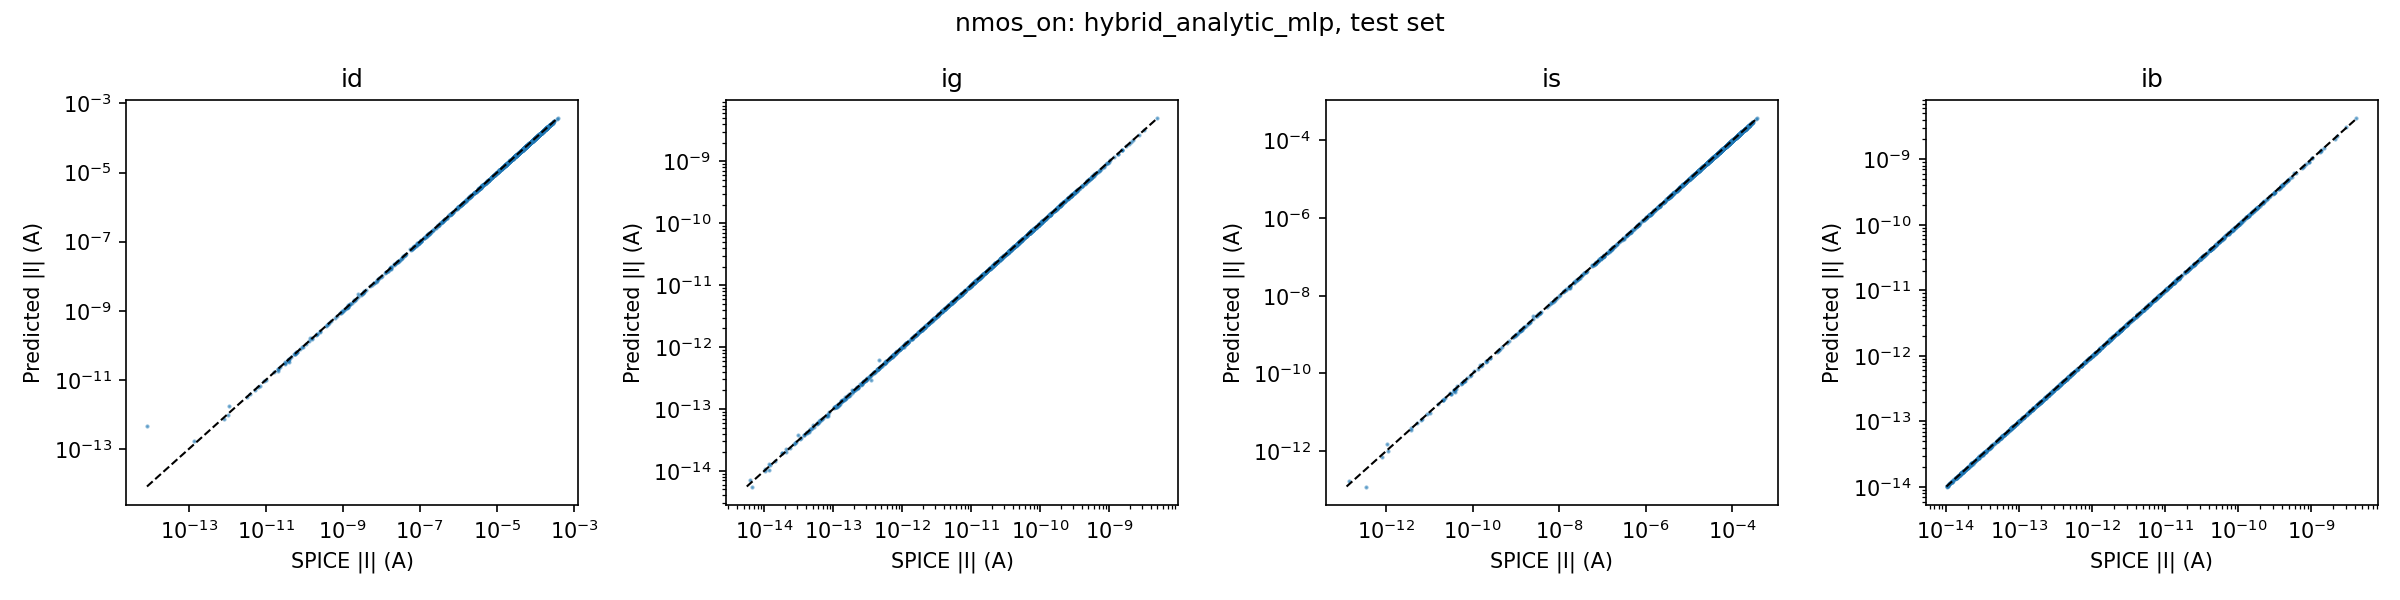
\includegraphics[width=0.78\textwidth]{figures/parity_nmos_on.png}\\[1mm]
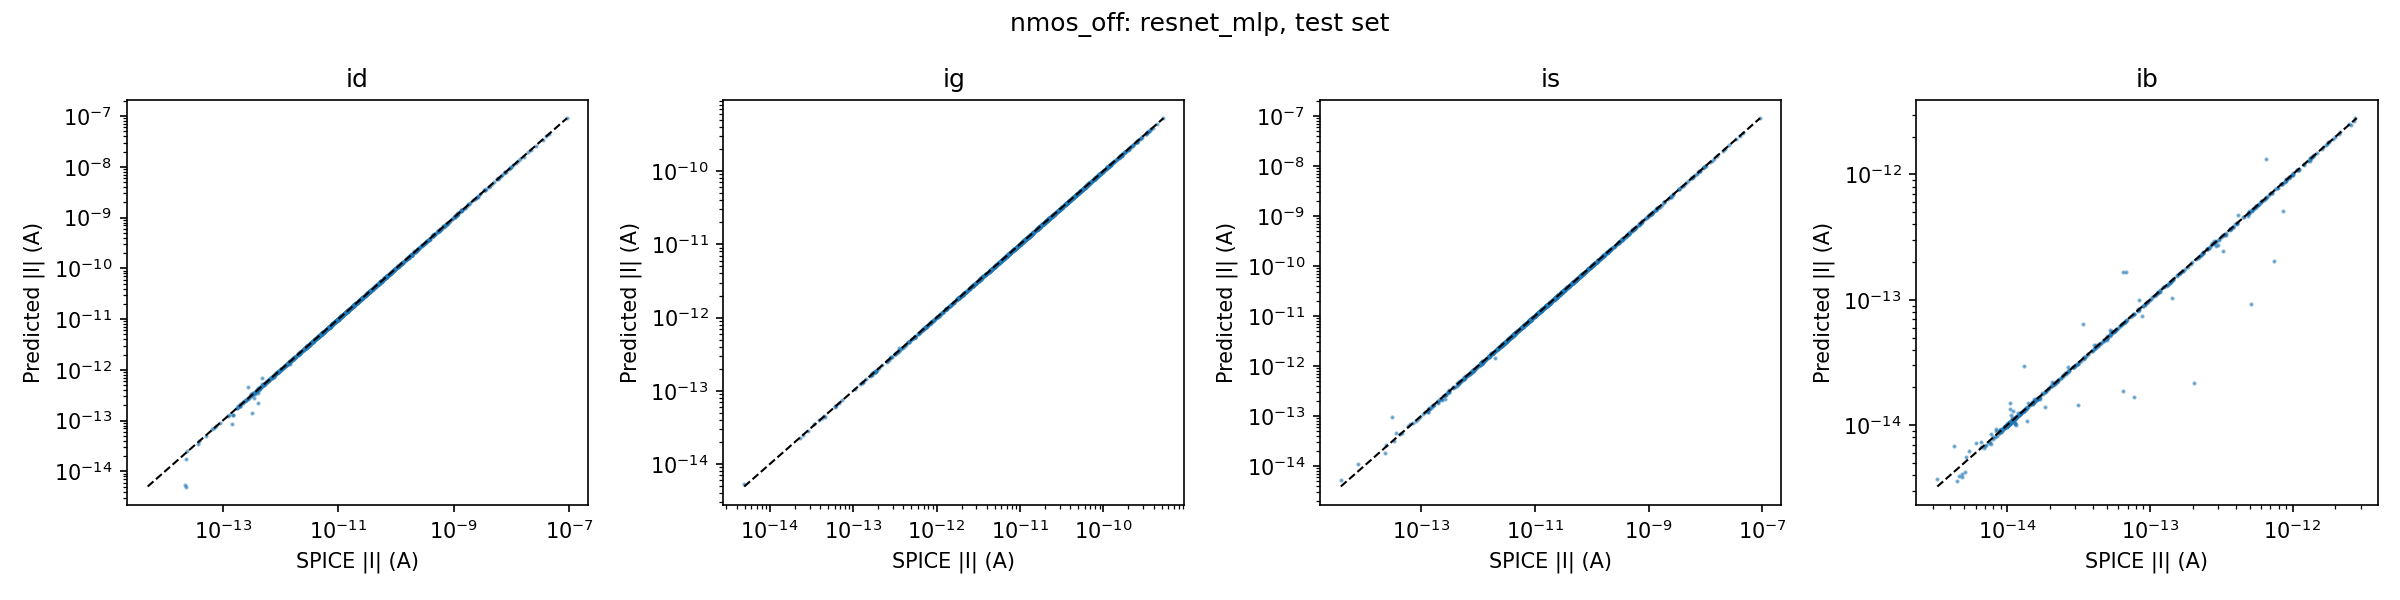
\includegraphics[width=0.78\textwidth]{figures/parity_nmos_off.png}\\[1mm]
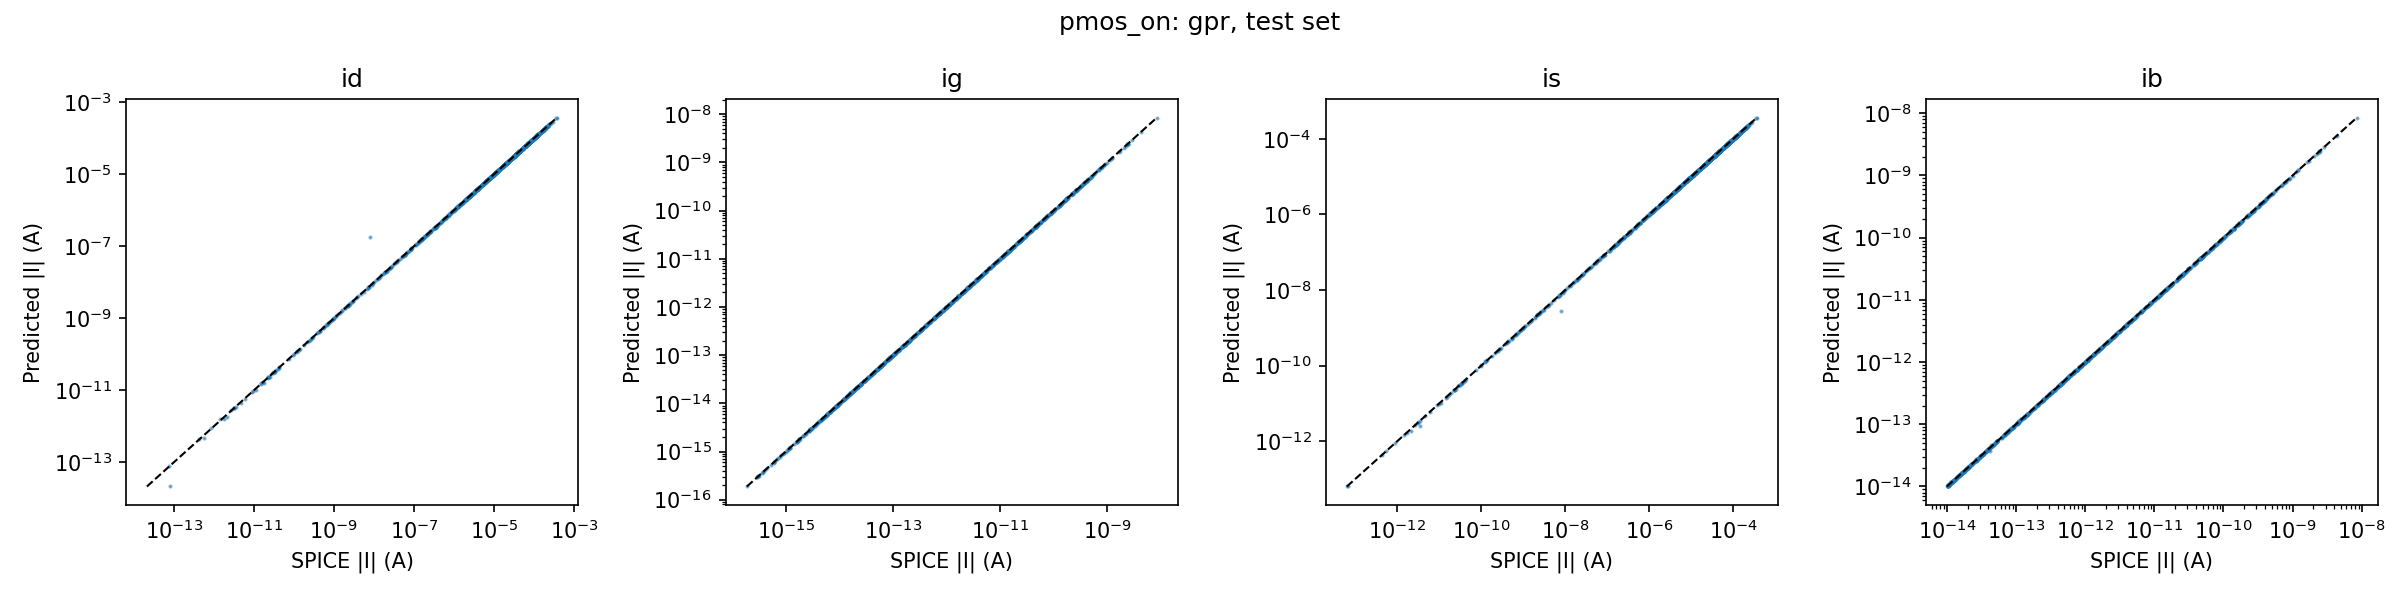
\includegraphics[width=0.78\textwidth]{figures/parity_pmos_on.png}\\[1mm]
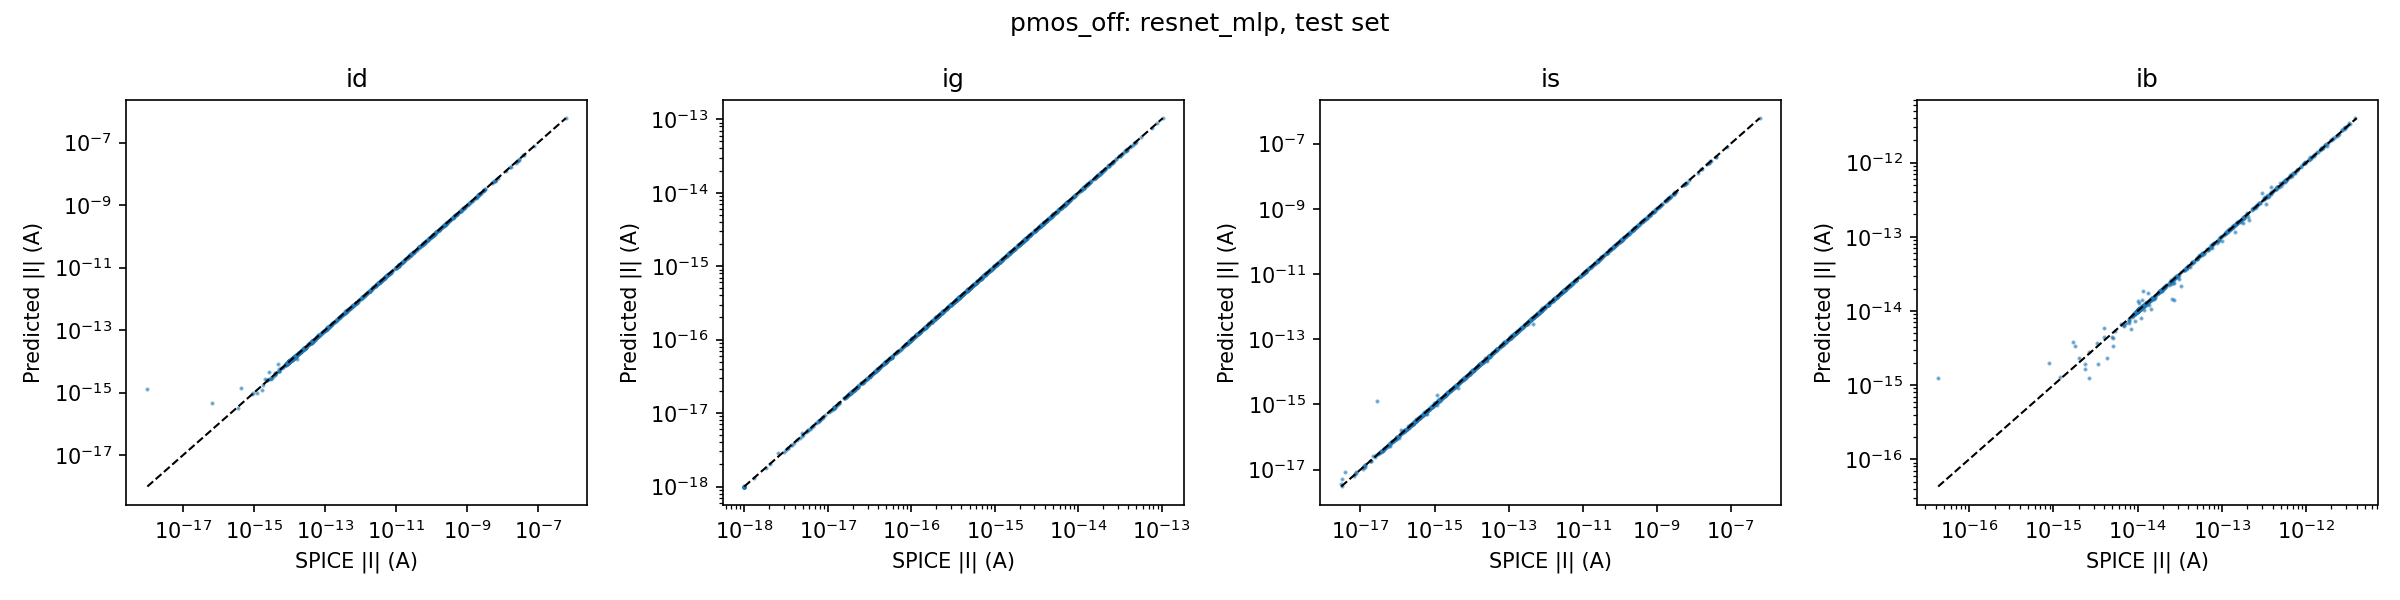
\includegraphics[width=0.78\textwidth]{figures/parity_pmos_off.png}
\caption{Chosen models on the test set: predicted versus SPICE $|I|$ for $i_d$, $i_g$, $i_s$, $i_b$ (log axes, dashed: prediction $=$ SPICE). From top: NMOS ON (hybrid), NMOS OFF (ResNet), PMOS ON (GPR), PMOS OFF (ResNet).}
\label{fig:parity}
% src: results/partA/parity_<case>.png
\end{figure*}

\end{document}
